
\fontsize{8pt}{10pt}\selectfont
\newgeometry{
    lmargin=0.2cm,
    rmargin=0.2cm,
    tmargin=0.2cm,
    bmargin=0.2cm,
}
\begin{landscape}
\begin{multicols*}{3}
    \section{Terminologia}
    \[
        \begin{cases}
            \dot{x}(t) = f(x(t),u(t),t) = Ax + bu\\
            y(t) = g(x(t),u(t),t) = cx +du
        \end{cases}
    \]
    \textbf{Stato}: le varie $x$;\newline
    \textbf{Uscita}: $y$;\newline
    \textbf{Sistema dinamico}: se la conoscenza degli ingressi su un intervallo di tempo
    non è sufficiente per determinare l’andamento delle uscite sullo stesso intervallo di tempo.\newline
    \textbf{Ordine del sistema}: numero di variabili di stato (quante $x$ ci sono).\newline
    \textbf{Lineare}: se $f$ e $g$ sono lineari in $x$ e in $u$ (non importa che lo siano in $t$), da notare che una funzione del tipo $x(t) \cdot u(t)$ non è lineare.\newline
    \textbf{Tempo invariante}: se in $f$ e $g$ non compare esplicitamente $t$;\newline
    \textbf{Strettamente proprio}: se in $g$ non compare $u$.\newline
    \textbf{SISO}: single input, single output; cioè se $u$ e $y$ sono scalari.
    \section{Equilibrio}
    \subsection{Caso generale}
    Dato l'ingresso costante $u = \bar{u}$ e detto $\bar{x}$ l'equilibrio cercato, in generale si ha:\newline
    \textbf{TC}: Soluzioni di $f(\bar{x},\bar{u}) = 0$.\newline
    \textbf{TD}: Soluzioni di $f(\bar{x}, \bar{u}) = \bar{x}$.\newline
    Per trovare le uscite di equilibrio $\bar{y}$ è sufficiente applicare gli stati di equilibrio $\bar{x}$ trovati all'uscita e vedere se l'espressione non perde senso e se produce soluzioni reali.
    \subsection{Caso lineare}
    Se il sistema è lineare:\newline
    \textbf{TC, LTI}: Soluzioni di $A\bar{x} + b \bar{u} = 0$.\newline
    \textbf{TD, LTI}: Soluzioni di $A\bar{x} + b \bar{u} = \bar{x}$.\newline
    Se esiste $\bar{x}$, allora per forza esiste un uscite di equilibrio $\bar{y}$
    \subsection{Caso non lineare}
    Se il sistema \textbf{non} è lineare:\newline
    L'uscita $\bar{y}$ potrebbe non avere senso per gli equilibri $\bar{x}$ trovati. 
    \newpage\section{Movimento}
    \subsection{Formula di Lagrange TC, LTI}
    \textbf{Per lo stato}:
    \[
            \begin{split}
            x(t) &= x_L(t) + x_F(t) =\\
            &=e^{At} x(0) + \int_{0}^{t}e^{A(t-\tau)}bu(\tau)d \tau
            \end{split}
    \]
    \[
        \begin{cases}
            x_L(t) = e^{At} x(0)\\
            x_F(t) = \int_{0}^{t}e^{A(t-\tau)}bu(\tau)d \tau
        \end{cases}
    \]
    \textbf{Per l'uscita}:
    \[
            \begin{split}
            y(t) 1 &= y_L(t) + y_F(t) =\\
            &= ce^{At}x(0) + c \int_{0}^{t}e^{A(t-\tau)}bu(\tau)d \tau + du(t)
            \end{split}
    \]
    \[
        \begin{cases}
            y_L(t) = ce^{At}x(0)\\
            y_F(t) = c \int_{0}^{t}e^{A(t-\tau)}bu(\tau)d \tau + du(t)
        \end{cases}
    \]
    \subsection{Formula di Lagrange TD, LTI}
    \textbf{Per lo stato}:
    \[
            \begin{split}
            x(k) &= x_L(k) + x_F(k) =\\
            &=A^k x(0) + \sum_{l=0}^{k-1}A^{k-l-1}bu(l)
            \end{split}
    \]
    \[
        \begin{cases}
            x_L(k) A^k x(0)\\
            x_F(k) \sum_{l=0}^{k-1}A^{k-l-1}bu(l)
        \end{cases}
    \]
    \textbf{Per l'uscita}:
    \[
        \begin{split}
            y(k) &= y_L(k) + y_F(k) =\\
            &= cx(k)+du(k) = \\
            &=cA^k x(0) + c\sum_{l=0}^{k-1}A^{k-l-1}bu(l) + du(k)
        \end{split}
    \]
    \[
        \begin{cases}
            y_L(k) = cA^k x(0)\\
            y_F(k) = c\sum_{l=0}^{k-1}A^{k-l-1}bu(l) + du(k)
        \end{cases}
    \]
    \subsection{Esponenziale di matrice (con $A$ diagonalizzabile)}
    $A$ è \textbf{diagonalizzabile} se:
    \begin{itemize}
        \item il numero di autovalori contati con la loro molteplicità è pari all’ordine della matrice;
        \item la molteplicità geometrica di ciascun autovalore coincide con la relativa molteplicità algebrica;
        \item una matrice quadrata di ordine $n$ che ammette esattamente $n$ autovalori distinti è sicuramente diagonalizzabile.
    \end{itemize}
    Per calcolare $e^{At}$ si seguono i seguenti passaggi:
    \begin{itemize}
        \item Calcolare gli autovalori di $A$ (risolvere $det[A-\lambda I] = 0$, oppure se matrice triangolare, gli autovalori sono sulla diagonale);
        \item Calcolare gli autovettori corrsipondenti per ogni autovalore \newline (risolvere $[A-\lambda_i I] \cdot \left[\begin{matrix}
            x\\y
        \end{matrix}\right] = \left[\begin{matrix}
            0\\0
        \end{matrix}\right]$);
        \item definire la matrice diagonalizzante $T$ come l'accostamento degli autovettori trovati (ricordando l'ordine) e calcolare $T^{-1}$. Per l’inversa della generica matrice $T$ 2x2 si moltiplica $\frac{1}{det(T)}$ per la matrice ottenuta da $T$ scambiando di posto i termini sulla diagonale principale e invertendo
        il segno dei termini sulla diagonale secondaria.
        \item notare che $T^{-1} A T = D = $ matrice con gli autovalori di $A$ lungo la diagonale nell'ordine in cui compaiono gli autovettori in $T$.
        \item Calcolare $e^{At}$:\newline
        $e^{At} = e^{TDT^{-1} t} = T e^{Dt} T^{-1} = \dots$
    \end{itemize}
    \subsection{Movimento libero con Jordanizzazione (con $A$ non diagonalizzabile)}
    Se la matrice $A$ non è diagonalizzabile calcolare $e^{At}$ col metodo spiegato prima non è fattibile, piuttosto usare questo procedimento:
    \begin{itemize}
        \item Calcolare gli autovalori di $A$;
        \item Se ci sono autovalori coincidenti, cercare di calcolare gli autovettori corrispondenti (risulterà possibile se e solo se la molteplicità geometrica è pari alla molteplicità algebrica). Se non si riescono a trovare abbastanza autovettori bisogna usare la Jordanizzazione, vediamo come fare.
        \item per ogni autovalore multiplo, chiamiamolo per semplicità $\lambda$, bisogna cercare gli autovettori generalizzati corrispondenti e da questi creare una catena di autovettori.
        \item Il primo autovettore generalizzato è quello classico calcolato come soluzione di $(A-\lambda I_n) x = 0$.
        \item Il secondo autovettore generalizzato è calcolato come soluzione di $(A-\lambda I_n)^2 x = 0$, dove per $(A-\lambda I_n)^2$ è sufficiente fare il prodotto della matrice per sè stessa. E' tipico che un autovettore generalizzato abbia come soluzione un insieme di soluzioni, se siamo al secondo, tipicamente ce ne saranno due.
        \item Tutti gli altri autovettori generalizzati si calcolano allo stesso modo incrementando di uno l'esponente ogni volta.
        \item Una volta trovati tutti gli autovettori generalizzati bisogna fare una catena di autovettori.
        \item A partire dall'ultimo autovettore generalizzato trovato si sceglie un vettore, che chiamo qua $v_n$, fra quelli della soluzione che non appartenga all'insieme dei vettori soluzione dell'autovettore generalizzato precedente. Una volta selezionato, si trova l'autovettore precedente come $v_{n-1} = (A- \lambda I_n)v_n$. E si prosegue così anche per quello prima: $v_{n-2} = (A-\lambda I_n) v_{n-1}$.
        \item una volta terminata la catena di autovettori, questi, accostati in colonna, rappresentano la matrrice jordanizzante $P$, tale che $P^{-1} A P = J =$ matrice in forma canonica di Jordan.
    \end{itemize}
    Vediamo ora come trovare la forma canonica di Jordan della matrice $A$ nel caso 2x2:
    \begin{itemize}
        \item se $\lambda_1 \neq \lambda_2$, allora la matrice di Jordan è la matrice diagonale classica;
        \item se $\lambda_1 = \lambda_2$:
        \begin{itemize}
            \item se ammette due autovettori, allora siamo ancora nella matrice diagonale classica;
            \item se la matrice ammette un solo autovettore, allora abbiamo una matrice di Jordan: $\left[\begin{matrix}
                \lambda & 1\\ 0 & \lambda
            \end{matrix}\right]$
        \end{itemize}
    \end{itemize}
    Vediamo ora come trovare la forma canonica di Jordan della matrice $A$ nel caso 3x3:
    \begin{itemize}
        \item se $\lambda_1 \neq \lambda_2 \neq \lambda_3$ allora la matrice di jordan è la solita diagonale;
        \item se $\lambda_1 = \lambda_2 = \lambda$ e $\lambda_3 \neq \lambda$ allora:
        \begin{itemize}
            \item se $\lambda$ ammette due autovettori, allora siamo alla diagonale solita;
            \item se $\lambda$ non ammette due autovettori, allora la matrice di Jordan:$\left[\begin{matrix}
                \lambda & 1 & 0 \\
                0 & \lambda & 0\\
                0 & 0 & \lambda_3
            \end{matrix}\right]$
        \end{itemize}
        \item se $\lambda_1 = \lambda_2 = \lambda_3 = \lambda$, allora:
        \begin{itemize}
            \item se $\lambda$ ammette tre autovettori, allora siamo alla solita diagonale;
            \item se $\lambda$ ammette due autovettori, allora la matrice di jordan: $\left[\begin{matrix}
                \lambda & 1 & 0 \\
                0 & \lambda & 0\\
                0 & 0 & \lambda
            \end{matrix}\right]$
            \item se $\lambda$ ammette un solo autovettore, allora la matrice di Jordan: $\left[\begin{matrix}
                \lambda & 1 & 0 \\
                0 & \lambda & 1\\
                0 & 0 & \lambda
            \end{matrix}\right]$
        \end{itemize}
    \end{itemize}
    Una volta determinate le matrici jordanizzanti e la matrice di jordan si può proseguire a calcolare il movimento libero:
    \begin{itemize}
        \item partendo dal sistema $\dot{x} = A x$, il movimento libero è $x_L(t) = e^{At}x(0)$;
        \item per prima cosa si fa un cambio di variabile: $\bar{x} = P^{-1}x$, per cui il sistema diventa $P \bar{\dot{x}} = A P \bar{x}$, e spostando $P$ otteniamo $\bar{\dot{x}} = P^{-1} A P \bar{x} = J \bar{x}$.
        \item Siccome la matrice di Jordan è triangolare alta si può ora evitare di usare le matrici e trasformare il sistema in forma scalare. Per esempio, ipotizzando $J = \left[\begin{matrix}
            a & b \\ 0 & c
        \end{matrix}\right]$ otteniamo il sistema $\begin{cases}
            \bar{\dot{x}}_1 = a \bar{x}_1 + b \bar{x}_2\\
            \bar{\dot{x}}_2 = c \bar{x}_2
        \end{cases}$.
        \item la seconda equazione contiene solo $\bar{x}_2$ e quindi il suo movimento libero è $\bar{x}_2 = e^{ct}\bar{x}_2(0)$
        \item Il movimento libero della prima equazione è ora calcolabile come moviemento completo (!) considerando $b \bar{x}_2$ come fosse un ingresso: $\bar{x}_1 = e^{at}\bar{x}_1(0) + \int_{0}^{t} e^{a(t-\tau)} b \bar{x}_2(\tau) d \tau$ e sostituendo il $\bar{x}_2(\tau)$ trovato al punto precedente.
        \item Abbiamo ora trovato le due componenti del vettore movimento libero per $\bar{x}_L$, bisogna però sostituire i valori iniziali $\bar{x}(0) = P^{-1}x(0)$, e, infine, non ci resta che tornare alla variabile iniziale: $x_L (t) = P \bar{x}_L$
    \end{itemize}
    \subsection{Osservazioni}
    \begin{itemize}
        \item Se è richiesto il calcolo del movimento dell'uscita, è sufficiente calcolare il movimento dello stato e sostituirlo nell'equazione dell'uscita del sistema.
        \item Se gli autovalori di $A$ sono numeri complessi: una volta ricondotti i numeri complessi in $x_L$ alla loro forma trigonometrica ($cos(\theta) + i sin(\theta) = e^{i \theta}$), si prende la sola parte reale, l'unità immaginaria deve scomparire.
        \item Alla fine in $x_L$ devono comparire somme di termini del tipo $e^{\alpha t} cos(\omega t)$ e/o $e^{\alpha t} sin(\omega t)$, dove $\alpha$ e $\omega$ sono rispettivamente perti reali e immaginarie di autovalori di $A$. In realtà si possono trovare anche altri termini, ma in via generale se si trova un coefficiente del tempo all'esponente che non è parte reale di nessun autovalore di $A$, il risultato è certamente errato.
        \item Il movimento libero dipende linearmente solo dallo stato iniziale e non dall’ingresso, il movimento forzato dipende linearmente solo dall’ingresso e non dallo stato iniziale.
    \end{itemize}
    \newpage\section{Stabilità}
    \begin{itemize}
        \item Tutti gli equilibri hanno le stesse caratteristiche di stabilità.
        \item Nei sistemi lineari (tempo invarianti) la stabilità è una proprietà del sistema, e non una proprietà dell’equilibrio. 
        \item Nei sistemi \textbf{asintoticamente stabili} i movimenti \textbf{liberi} di stato e di uscita tendono a $0$ per $t \rightarrow \infty$ (dimenticano lo stato inizile, movimento libero trascurabile a lungo andare) qualunque sia lo stato iniziale, mentre se li si sottopone a ingresso costante i movimenti (complessivi, non solo liberi) di stato e di uscita tendono ai medesimi valori costanti qualunque sia lo stato iniziale;
        \item Nei sistemi \textbf{instabili} il movimento \textbf{libero} di stato e di uscita diverge a patto di alcune eccezioni. Diverge in generale anche il movimento (complessivo, non solo libero) di stato e di uscita a frornte di un ingresso costante.
        \item nei sistemi \textbf{semplicemente stabili} i movimenti \textbf{liberi} di stato e di uscita nè divergono nè tendono a zero e il loro comportamento asintotico non è lo stesso per qualunque stato iniziale.
    \end{itemize}
    \subsection{Criteri di stabilità}
    \textbf{tempo continuo}:
    \begin{itemize}
        \item Tutti gli autovalori di $A$ hanno $Re < 0 \Longleftrightarrow $ sistema AS;
        \item Almeno un autovalore di $A$ ha $Re > 0 \Longrightarrow$ sistema I;
        \item Tutti gli autovalori di $A$ hanno $Re \leq 0$ e ne esiste almeno uno con $Re = 0$ $\Longrightarrow$ $\begin{cases}
            \text{sistema I;}\;\\
            \text{oppure sistema S, ma non AS.}\;
        \end{cases}$. \newline
        Per capire se si tratta di un sistema stabile o instabile bisogna andare a calcolare il movimento libero per un generico ingresso $x(0)$ e vederne il comportamento per $t \rightarrow \infty$. Se il movimento libero rimane sempre limitato allora il sistema è stabile, se il movimento libero diverge (anche una sola delle componenti del movimento libero) allora il sistema è instabile. \newline
        Esiste anche un altro metodo: guardando la matrice di Jordan, se il più grande miniblocco di Jordan ha dimensione $1$ allora il sistema è stabile, altrimenti è instabile. Un buon metodo per ricordarlo è usare i seguenti due esempi che abbiamo visto a esercitazione:
        \[
            \left[\begin{matrix}
                0 & 0 \\
                0 & 0
            \end{matrix}\right] \;\;\text{due miniblocchi di dimensione 1, quindi S}\;
        \]
        \[
            \left[\begin{matrix}
                0&1\\
                0&0
            \end{matrix}\right] \;\; \text{un miniblocco di dimensione 2, quindi I}\;
        \]
    \end{itemize}
    \textbf{tempo discreto}:
    \begin{itemize}
        \item Tutti gli autovalori di $A$ hanno $|\lambda_i| < 1$ $\Longleftrightarrow$ sistema AS.
        \item Almeno un autovalore di $A$ con modulo $|\lambda_i| > 1$ $\Longrightarrow$ sistema I.
        \item Tutti gli autovalori di $A$ hanno $|\lambda_i| \leq 1$ e ne esiste almeno uno tale che $|\lambda_1| = 1$ $\Longrightarrow$ $\begin{cases}
            \text{sistema I;}\;\\
            \text{oppure sistema S, ma non AS.}\;
        \end{cases}$. \newline
        Per capire se il sistema è instabile o stabile nell'ultimo punto guarda il caso a tempo continuo.
    \end{itemize}
    \textbf{oss.} Errore tipico: Nel caso a tempo continuo si guarda la parte reale degli autovalori, nel caso a tempo discreto si guarda il modulo (!) degli autovalori.
    \subsection{Criteri di stabilità dedotti dalla matrice $A$}
    \begin{itemize}
        \item Se il sistema è asintoticamente stabile, allora $tr(A)$ è negativa, ma non vale il viceversa.
        \item se $det(A) = 0$ esiste $S_i = 0$ $\Longrightarrow$ no AS.
        \item se $tr(A) >0$ $\Longrightarrow$ sistema I.
        \item se $tr(A) = 0$ $\Longrightarrow$ no AS.
        \item Se $Re(S_i)<0$ per ogni $i$ (cioè se il sistema è asintoticamente stabile), allora i coefficienti di $\Pi(S)$ sono tutti concordi e non nulli \newline
        \textbf{oss.} Errore tipico: il viceversa vale solo per polinomi del secondo ordine.
    \end{itemize}
    \textbf{oss.} Per stabilire se un sistema è asintoticamente stabile abbiamo due possibilità: per prima cosa con i primi due dei tre criteri appena esposti stabiliamo se non è asintoticamente stabile, altrimenti, se non abbiamo avuto fortuna con questi criteri, usiamo il criterio di Routh. Un caso particolare è rappresentato dai polinomi di secondo ordine, in cui possiamo evitare di usare Routh e usare il terzo criterio appena visto.
    \subsection{Routh}
    \[
        \Pi(s) = a_0s^n + a_1 s^{n-1} + \dots + a_{n-1}s + a_n
    \]
    Prime due righe
    \[
        \begin{matrix}
            a_0 & \;\;\;\;\;\; a_2 & \;\;\;\;\;\;\dots\\
            \;\;\downarrow & \nearrow \;\; \downarrow & \nearrow \;\; \downarrow\\
            a_1 & \;\;\;\;\;\; a_3 & \;\;\;\;\;\;\dots 
        \end{matrix}
    \]
    a seconda che il numero di termini sia pari (le due righe sono di pari lunghezza) o dispari (la prima riga ha un termine in più della seconda, per cui si aggiunge uno $0$) l'ultima colonna può terminare in due modi:
    \[
        \begin{matrix}
            \dots & a_{n-1}\\
            \;\\
            \dots & a_n
        \end{matrix}\;\;\;\;\;\;\;\;\;\;\; \text{oppure}\;\;\;\;\;\;\;\;\;\;\; \begin{matrix}
            \dots &a_n\\
            \;\\
            \dots & 0 
        \end{matrix}
    \]
    In totale, considerando anche le prime due righe, ci sono $n+1$ righe.\newline
    Ogni riga dalla terza in poi dipende dalle due precedenti seguendo una regola:
    \[
        \begin{matrix}
            h_1 & h_2 & h_3 &\dots\\
            \;\\
            q_1 & q_2 & q_3 & \dots\\
            \;\\
            w_1 & w_2 & w_3 & \dots
        \end{matrix}
    \]
    prese due generiche righe ($h_i$ e $q_i$), i termini della riga successiva ($w_i$) si costruiscono come $w_i = - \frac{1}{q_1} det\left[\begin{matrix}
        h_1 & h_{i+1} \\
        q_1 & q_{i+1}
    \end{matrix}\right]$.\newline
    Se manca un termine in una delle righe precedenti ($h$ e $q$) si assume nullo.\newline
    Se troviamo un elemento nullo in prima colonna, ci si ferma, sicuramente il sistema non è asintoticamente stabile, e siamo in presenza di un caso particolare che non ci permette di calcolare la tabella di Routh.\newline
    \newline
    Un sistema dinamico con polinomio caratteristico $\Pi(s)$ è asintoticamente stabile se e solo se tutti gli elementi della prima colonna della tabella di Routh sono concordi (e non nulli).
    \newpage\section{Linearizzazione}
    \subsection{Linearizzazione di sistemi tempo invarianti non lineari nell'intorno di un equilibrio}
    Dato il sistema dinamico 
    \[
        \begin{cases}
            \dot{x}_1(t) = f_1(x_1(t),x_2(t),\dots,x_n(t),u(t))\\
            \dot{x}_2(t) = f_2(x_1(t),x_2(t),\dots,x_n(t),u(t))\\
            \dots\\
            \dot{x}_n(t) = f_n(x_1(t),x_2(t),\dots,x_n(t),u(t))\\
            y(t) = g(x_1(t),x_2(t),\dots,x_n(t),u(t))
        \end{cases}
    \]
    e un suo equilibrio $(\bar{x}, \bar{u})$ a fronte dell'ingresso costante $\bar{u}$, tale sistema è approssimabile con uno lineare e stazionario ottenuto dall'espansione in serie delle $f_i$ e $g$ al prim'ordine:
    \[
        \begin{cases}
            \dot{\delta x} (t) = A \delta x(t) + b \delta u(t)\\
            \delta y (t) = c \delta x (t) + d \delta u (t)
        \end{cases}
    \]
    con:
    \[
        A = \left[\begin{matrix}
            \frac{\delta f_1 (x,u)}{\delta x_1}_{\bar{x}, \bar{u}} & \frac{\delta f_1 (x,u)}{\delta x_2}_{\bar{x}, \bar{u}} & \dots & \frac{\delta f_2 (x,u)}{\delta x_n}_{\bar{x}, \bar{u}}\\
            \frac{\delta f_2(x,u)}{\delta x_1}_{\bar{x}, \bar{u}} & \frac{\delta f_2(x,u)}{\delta x_2}_{\bar{x}, \bar{u}} & \dots & \frac{\delta f_1(x,u)}{\delta x_n}_{\bar{x}, \bar{u}}\\
            \dots & \dots & \dots & \dots\\
            \frac{\delta f_n(x,u)}{\delta x_1}_{\bar{x}, \bar{u}} & \frac{\delta f_n (x,u)}{\delta x_2}_{\bar{x}, \bar{u}} & \dots & \frac{\delta f_n (x,u)}{\delta x_n}_{\bar{x}, \bar{u}} 
        \end{matrix}\right]
    \]
    \[
        b = \left[\begin{matrix}
            \frac{\delta f_1 (x,u)}{\delta u}_{\bar{x}, \bar{u}}\\
            \frac{\delta f_2 (x,u)}{\delta u}_{\bar{x}, \bar{u}}\\
            \dots\\
            \frac{\delta f_n (x,u)}{\delta u}_{\bar{x}, \bar{u}}
        \end{matrix}\right]
    \]
    \[
        c = \left[\begin{matrix}
            \frac{\delta g(x,u)}{\delta x_1}_{\bar{x}, \bar{u}} &
            \frac{\delta g (x,u)}{\delta x_2}_{\bar{x}, \bar{u}} & 
            \dots &
            \frac{\delta g (x,u)}{\delta x_n}_{\bar{x}, \bar{u}}
        \end{matrix}\right]
    \]
    \[
        d = \frac{\delta g (x,u)}{\delta u}_{\bar{x}, \bar{u}}
    \]
    dove il pedice $|_{\bar{x}, \bar{u}}$ indica che sono derivate parziali valutate nell'equilibrio, e
    \[
        \delta x := x-\bar{x} \;\;\;\;\;\delta u := u- \bar{u} \;\;\;\;\; \delta y = := y- \bar{y}
    \]
    \subsection{Stabilità dell'equilibrio di sistemi tempo invarianti non lineari}
    La stabilità di un equilibrio si può studiare basandosi sul sistema linearizzato nell'intorno di quell'equilibrio:
    \begin{itemize}
        \item se il sistema linearizzato è AS, allora anche l'equilibrio è AS;
        \item se il sistema linearizzato è I, allora anche l'equilibrio è I;
        \item se il sistema linearizzato è S, allora nulla si può dire sulla stabilità dell'equilibrio, che in tal caso dipende da termini dello sviluppo in serie di $f$ di grado superiore a uno.
    \end{itemize}
    \textbf{oss.} Per i sistemi non lineari la stabilità non è una proprietà del sistema, quindi gli equilibri non condividono per forza la stessa "tipologia" di stabilità (AS/S/I). Di conseguenza è necessario analizzare la stabilità per ciascuno degli equilibri.
    \newpage\section{Trasformate e funzioni di trasferimento a TC}
    \subsection{Laplace}
    \[
        V(s) := \mathcal{L}[v(t)]
    \]
    \textbf{Calcolo della trasformata di Laplace}: $\mathcal{L}[\_\_] =  \int_{0}^{\infty}\_\_ e^{-st} dt$.\newline
    \textbf{Linearità}: $\mathcal{L}[\alpha_1 v_1(t) + \alpha_2 v_2(t)] = \alpha_1 \mathcal{L}[v_1(t)] + \alpha_2 \mathcal{L}[v_2(t)]$.\newline
    \textbf{Derivata}: $\mathcal{L}\left[ \frac{d v(t)}{dt} \right] = s \mathcal{L}[v(t)] - v(0)$.\newline
    \textbf{Integrale}: $\mathcal{L}\left[ \int_{0}^{t} v(\tau) d \tau \right] = \frac{1}{s} \mathcal{L}[v(t)]$.\newline
    \textbf{Ritardo}: $ \mathcal{L}[ v(t - \tau)] = e^{-s \tau} \mathcal{L}[v(t)]$ (spesso utilizzata al contrario per Heaviside: $\mathcal{L}^{-1}\left[\frac{N(s)}{D(s)}e^{-s \tau}\right] \rightarrow $ Heaviside di $\frac{N(s)}{D(s)}$ ottengo $y(t)$, poi con $e^{-s \tau}$ aggiungo ritardo $\tau$ e $\rightarrow  y(t- \tau)$).\newline
    \renewcommand{\arraystretch}{2}
    \begin{center}
        \begin{tabular}{ |c|c| } 
        \hline
        \;\;\;\;\;\;\;\;\;\;\;\;\;\;\;$v(t)$ \;\;\;\;\;\;\;\;\;\;\;\;\;\;\;& \;\;\;\;\;\;\;\;\;\;\;\;\;\;\;$V(s)$ \;\;\;\;\;\;\;\;\;\;\;\;\;\;\;\\ 
        \hline
        $k \cdot imp(t)$ & $k \cdot 1$ \\ 
        $k \cdot sca(t)$ & $k \cdot \frac{1}{s}$  \\ 
        $k \cdot ram(t) =k \cdot t \cdot  sca(t)$ & $k \cdot \frac{1}{s^2}$ \\
        $k \cdot e^{at}sca(t)$ & $k \cdot \frac{1}{s-a}$ \\ 
        $t^{n}\cdot e^{at}sca(t)$ & $\frac{n!}{(s-a)^{n+1}}$\\ 
        $\frac{1}{(n-1)!} t^{n-1}e^{-at}$ & $\frac{1}{(s+a)^n}$\\
        \hline
        \end{tabular}
    \end{center}
    \renewcommand{\arraystretch}{1}
    Notiamo che i segnali trigonometrici sono rappresentabili come esponenziali complessi, per esempio $sin(\omega t) = \frac{e^{j \omega t}- e^{-j \omega t}}{2j} \dots$ e così possiamo ricavare le \textbf{trasformate di Laplace di tutte le funzioni trigonometriche}.\newline
    \newline
    \textbf{Teorema del valore iniziale}:\newline
    Se $V(s) = \mathcal{L}[v(t)]$, allora $v(0) = \lim_{s\rightarrow +\infty} s \cdot V(s)$, oppure $v(0^+) = \lim_{s\rightarrow \infty}s \cdot V(s)$.\newline
    \newline
    \textbf{Teorema del valore finale}:\newline
    Se $V(s) = \mathcal{L}[v(t)]$ ed esiste $\lim_{t\rightarrow +\infty} v(t)$ o equivalentemente $V(s)$ ha solo poli con $Re< 0$ o nell'origine, allora $\lim_{t\rightarrow +\infty} v(t) = \lim_{s\rightarrow 0} s \cdot V(s)$.
    \subsection{Antitrasformazione con Heaviside}
    \[
        V(s) = \frac{N(s)}{D(s)}
    \]
    con $N,D$ polinomi in $s$.\newline
    Le radici di $N(s)$ sono gli \textbf{zeri}, mentre le radici di $D(s)$ sono i \textbf{poli}.\newline
    \begin{itemize}
        \item fattorizzare $D(s)$ in modo che sia espresso come prodotto di termini del tipo $(s-p)$ (\textbf{polo reale semplice}) oppure $(s-p)^n$ (\textbf{polo reale multiplo}):
        \item \textbf{polo reale semplice}: $\frac{N(s)}{\dots(s-p)\dots} = \dots + \frac{\alpha}{s-p} + \dots$.
        \item \textbf{polo reale multiplo}: $\frac{N(s)}{\dots (s-p)^n \dots} = \dots + \frac{\alpha_1}{s-p} + \frac{\alpha_2}{(s-p)^2} + \dots + \frac{\alpha_n}{(s-p)^n} + \dots$
    \end{itemize}
    A seguito della scomposizione l'antitrasformata è facilmente calcolabile come usando le trasformate notevoli.
    \subsection{Formula di Lagrange nel dominio delle trasformate}
    \textbf{Per lo stato}:
    \[
        X(s) = X_L(s) + X_F(s)
    \]
    \[
        \begin{cases}
            X_L(s) = (sI-A)^{-1} x(0)\\
            X_F(s) = (sI-A) ^{-1} b U(s)
        \end{cases}
    \]
    \textbf{Per l'uscita}:
    \[
        Y(s) = cX(s) + dU(s) = Y_L(s) + Y_F(s)
    \]
    \[
        \begin{cases}
            Y_L(s) = c(sI-A)^{-1} x(0)\\
            Y_F(s) = [c(sI-A)^{-1} b + d]U(s)
        \end{cases}
    \]
    Spesso può essere utile calcolare la $Y_F(s)$ a partire dall'equazione $\frac{Y(s)}{U(s)} = G(s)$
    \subsection{FdT}
    Il tipico sistema dinamico diventa:
    \[
        \begin{cases}
            s X(s) = AX(s) + b U(s)\\
            Y(s) = cX(s) + d U(s)
        \end{cases}
    \]
    \textbf{funzione di trasferimento}:
    \[
        G(s) := c(sI-A)^{-1} b + d = \frac{\tilde{N}(s)}{D(s)} + d = \frac{N(s)}{D(s)}
    \]
    Ricordiamo che $Y_F(s) = G(s) U(s)$.\newline
    \newline
    La funzione di trasferimento è un rapporto di polinomi il cui denominatore $D(s)$ è il polinomio caratteristico della matrice $A$, quindi i poli sono gli autovalori di $A$. In alcuni casi può capitare che alcuni termini del numeratore si semplifichino con alcuni temrini del denominatore e quindi non tutti gli autovalori di $A$ compaiano come poli.\newline
    Se e solo se $d=0$ (cioè se il sistema è strettamente proprio) abbiamo $G(s) = \frac{\bar{N}(s)}{D(s)}$ in cui il grado del numeatore è minore del grado del denominatore.\newline
    Altrimenti (se e solo se $d\neq 0$) abbiamo $G(s) = \frac{\bar{N}(s) + dD(s)}{D(s)} = \frac{N(s)}{D(s)}$, con $N(s) = \bar{N}(s) +dD(s)$, in cui il grado del numeratore è uguale al grado del denominatore.\newline
    \newline
    Calcolo della funzione di trasferimento con un ritardo: il calcolo è del tutto analogo al caso senza ritardo, basta ricordarsi di moltiplicare l'intera funzione di trasferimento per il termine trascendentale che ne rappresenta il ritardo, $G(s) = (c(sI-A)^{-1} b + d) e^{-a \tau}$.
    \newpage\section{Raggiungibilità e osservabilità}
    \subsection{Raggiungibilità}
    \textbf{Sistema raggiungibile se e solo se ($\Leftrightarrow$) $M_R$ è non singolare} (determinante diverso da zero), dove:
    \[
        M_R= \;\text{matrice di raggiungibilità}\; =\left[\begin{matrix}
            b & Ab & A^2 b & \dots & A^{n-1}b
        \end{matrix}\right]
    \] 
    dove nel caso SISO ogni suo termine è una matrice colonna $n$x$1$, e quindi in totale è una matrice $n$x$n$.
    \subsection{Osservabilità}
    \textbf{Sistema osservabile se e solo se ($\Leftrightarrow$) $M_O$ è non singolare} (determinante diverso da zero), dove:
    \[
        M_O = \left[\begin{matrix}
            c' & A'c' & \dots & (A^{n-1})' c'
        \end{matrix}\right]
    \]
    \subsection{Cancellazioni}
    Le parti non raggiungibili e/o non osservabili non sono presenti nella funzione di trasferimento.\newline
    Per cancellazione intendiamo il fatto che nel calcolo della funzione di trasferimento alcuni poli
    e zeri si possono cancellare fra di loro, e questi rappresentano proprio le parti non raggiungibili
    e/o non osservabili.\newline
    \newline
    Una calcellazione è \textbf{critica} se avviene al di fuori della regione di asintotica stabilità (a tempo continuo significa che se l'autovalore è cancellato, non ha la parte reale negativa).\newline
    Poichè i poli di $G(s)$ sono gli autovalori della parte raggiungibile e osservabile del sistema, perchè si possa studiare la stabilità (asintotica) del sistema usando $G(s)$, non vi devono essere cancellazioni critiche.
    \newline
    \newline
    Per capire se un FdT ha parti nascoste basta controllare se una radice del numeratore azzera anche il denominatore o se una radice del denominatore annulla il numeratore. 
    \section{Realizzazione}
    Metodo per la \textbf{forma canonica di raggiungibilità} (realizzazione sempre raggiungibile).
    se il grado del numeratore è uguale al grado del denominatore si fa la divisione e si ottiene $G(s) = d + \frac{N(s)}{D(s)}$, da cui si ricava il valore $d$. A questo punto riscriviamo la frazione $\frac{N(s)}{D(s)} = \frac{ b_1 s^{n-1} + b_2 s^{n-2} + \dots + b_n }{ s^n + a_1 s^{n-1} + \dots + a_n }$ e scriviamo le $A, b$ e $c$:
    \[
        A=\left[\begin{matrix}
            0 & 1 & 0 & \dots & 0 \\
            0 & 0 & 1 & \dots & 0 \\
            \dots & \dots &\dots&\dots&\dots\\
            0 & 0 & 0 & \dots & 1\\
            -a_n & -a_{n-1} & \dots & \dots & -a_1
        \end{matrix}\right]
    \]
    \[
        b=\left[\begin{matrix}
            0\\\dots\\0\\1
        \end{matrix}\right]
    \]
    \[
        c=\left[\begin{matrix}
            b_n & b_{n-1} & \dots & b_1
        \end{matrix}\right]
    \]
    \textbf{oss.} la presenza di una cancellazione ci impone il fatto che la realizzazione
    $ (A, b, c, d)$ non può essere raggiungibile e osservabile contemporaneamente. Quindi siccome facciamo una realizzazione raggiungibile, sarà sicuramente non osservabile.
    \section{Schemi a blocchi}
    \textbf{Blocchi in serie}: $u \rightarrow [G_1] \rightarrow  [G_2] \rightarrow y$, con $G_1 = \frac{N_1}{D_1}$ e $G_2 = \frac{N_2}{G_2}$: $\frac{Y}{U} = G_2G_1 = \frac{N_1N_2}{D_2D_1}$.\newline 
    Gli autovalori del sistema complessivo sono i $\{$ poli di $G_1\} U \{$ poli di $G_2\}$.\newline
    $G_1$ e $G_2$ (entrambi) asintoticamente stabili è condizione neccessaria e sufficiente ($\Leftrightarrow$) per avere un sistema complessivo asintoticamente stabile.\newline
    \newline
    \textbf{Blocchi in parallelo}: con $G_1 = \frac{N_1}{D_1}$ e $G_2 = \frac{N_2}{G_2}$: $\frac{Y}{U} = G_1 + G_2 = \frac{N_2D_1 + N_1 D_2}{D_1D_2}$.\newline
    Quindi gli autovalori del sistema complessivo sono $\{\text{poli di $G_1$}\} U \{\text{poli di $G_2$}\}$.\newline
    $G_1$ e $G_2$ (entrambi) asintoticamente stabili è condizione necessaria e sufficiente ($\Leftrightarrow$) per avere un sistema complessivo asintoticamente stabile.\newline
    \newline
    \textbf{Blocchi in retroazione}: con $G_a$ blocco di andata e $G_r$ blocco di retroazione: $\frac{Y}{U} = \frac{G_a}{1 + G_aG_r} = \frac{\text{"andata"}}{1+ \text{"anello"}} = \frac{N_aD_r}{D_aD_r +N_aN_r}$. \newline
    $G_a$ e $G_r$ asintoticamente stabili nè occorrono nè bastano per avere un sistema complessivo asintoticamente stabile.
    \subsection{Costruzione dello schema a blocchi}
    \textbf{Primo metodo (analitico)}
    \begin{itemize}
        \item Si trasforma il sistema $\begin{cases}
            \dot{x} = A x + bu\\ y = cx +d
        \end{cases}$ secondo Laplace: $\begin{cases}
            s X = A X + b U\\ Y = c X + d
        \end{cases}$;
        \item Si esprime il sistema secondo le variabili di stato e secondo l'uscita:$\begin{cases}
            X = \;\text{qualcosa}\;\\ Y = \;\text{qualcosa}\;
        \end{cases}$;
        \item Ora è facile ricostruire lo schema a blocchi.
    \end{itemize}
    \textbf{Secondo metodo (Funzione di trasferimento)}
    \begin{itemize}
        \item Si calcola la funzione di trasferimento $G(s)$;
        \item Ricordando che $Y = G(s) U$ possiamo scrivere il sistema a blocchi come: $Y \longrightarrow \left[G(s)\right] \longrightarrow U$
    \end{itemize}
    \textbf{Terzo metodo (Integratori)}\newline
    Ricordiamo che la funzione integrale nel dominio delle trasformate è rappresentato dall'aggiunta di un termine $\frac{1}{s}$ (\textbf{es.} $y(t) = \int_{0}^{t}u(\tau)d \tau \Rightarrow Y(s) = \frac{1}{s} U(s)$ ).\newline
    Il termine $\frac{1}{s}$ è la funzione di trasferimento dell'integratore.
    \begin{itemize}
        \item Si disegnano $n$ blocchi integratori $\frac{1}{s}$ quante sono le $n$ variabili di stato del sistema;
        \item Per ciascuno di questi blocchi $n$ si mette come ingresso la variabile derivata ($\dot{x}_n$) e come uscita la variabile semplice ($x_n$);
        \item Osservando le matrici $A$ e $b$ si compongono con dei nodi sommatori i vari $\dot{x}_1, \dots, \dot{x}_n$;
        \item Infine osservando le matrici $c$ e $d$ si compone l'uscita.
    \end{itemize}
    [immagine dagli appunti del prof]
    \begin{center}
        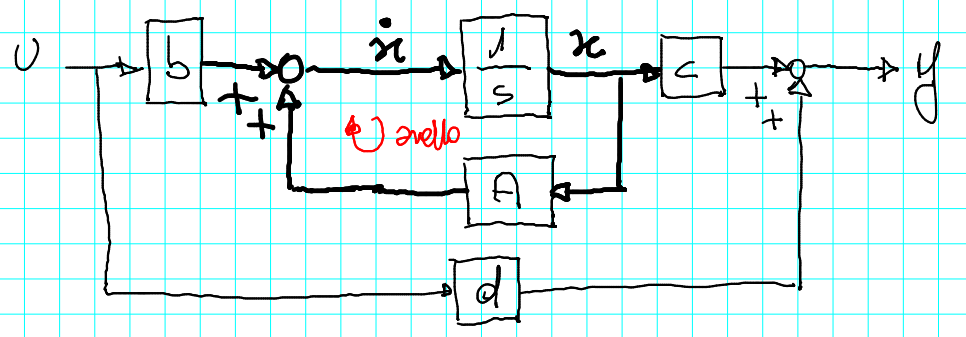
\includegraphics[height=2cm]{../lezione8/img1.PNG}
    \end{center}
    Rappresentazioen di dove solitamente si inseriscono i valori delle matrici del sistema all'interno dello schema a blocchi sviluppato con l'integratore.
    \section{Risposta esponenziale}
    Quindi \textbf{in generale} con $u(t) = U e^{\lambda t}$ (con $U$ un numero qualunque che semplicemente amplifica l'esponenziale), se $\lambda$ non è autovalore di $A$, allora esiste uno e uno solo 
    \[
        x(0) = (\lambda I - A)^{-1}b U
    \] tale che 
    \[
        \begin{cases}
            x(t) = (\lambda I -A)^{-1} b U e^{\lambda t}\\
            y(t) = cx(t) + du(t) =  [c(\lambda I -A)^{-1} b + d] U e^{\lambda t} = G(\lambda) u(t)
        \end{cases}
    \]
    Se, inoltre, il sistema è asintoticamente stabile, allora qualunque sia lo stato iniziale $x(0)$, l'uscita tenderà a $y(t) \rightarrow G(\lambda) u(t)$ per $t \rightarrow  \infty$.
    \section{Risposta sinusoidale}
    Dato il sistema dinamico LTI a TC, SISO $\begin{cases}
        \dot{x} = Ax +bu\\ 
        y = cx +du
    \end{cases}$, detta $G(s)$ la sua funzione di trasferimento e considerato l'ingresso $u(t) = U sin(\omega t)$ per $t\geq 0$:
    \begin{itemize}
        \item Se $\mp j \omega$ non sono autovalori di $A$, allora esiste uno e uno solo stato iniziale $x(0)$ tale che $y(t) = |G(j \omega)| U sin(\omega t + arg(G(j \omega)))$ per $t\geq 0$. (Se $\mp j \omega$ sono autovalori di $A$, allora si verifica un fenomeno di risonanza, che però non è argomento di questo corso).
        \item Se INOLTRE il sistema è asintoticamente stabile, allora qualunque sia lo stato iniziale, l'uscita  tenderà a $y(t) \rightarrow |G(j \omega) U sin( \omega t + arg(G(j \omega)))$ per $t \rightarrow  \infty$
    \end{itemize}
    \textbf{definizione}:  Data una funzione di trasferimento $G(s)$, la sua restrizione all'asse immaginario positivo $J^+$, cioè $G(j \omega)$ con $\omega \geq 0$, si dice \textbf{risposta in frequenza} (RF) di $G(s)$.
    \newpage\section{Diagramma di Bode}
    $x_{dB} = 20 log_{10}|x|$\newline
    \[
        G(s) = \frac{\mu}{s^g} \cdot \frac{(1 + s \tau_1)(1 + s \tau_2)\dots}{(1 + s t_1)(1 + s t_2)\dots} \cdot \frac{(1 + 2 \frac{\zeta}{\sigma_n}s + \frac{1}{\sigma_n^2}s^2)\dots}{(1 + 2 \frac{\xi}{\omega_n} s + \frac{1}{\omega_n^2}s^2)\dots}
    \]
    \[
        \begin{matrix}
            G_a(s) = \mu & \;\; & G_c(s) = 1+ s t\\
            G_b(s) = \frac{1}{s^g} & \;\; & G_d(s) = 1 + 2 \frac{\xi}{\omega_n}s + \frac{1}{\omega_n^2}s^2
        \end{matrix}
    \]
    \subsection{Metodo di tracciamento}
    Per prima cosa si ricavano i valori di $\mu$, $g$, poi si ricavano tutte le frequenze d'angolo (modulo delle radici di ogni termine al numeratore e al denominatore, escluse quelle in $s=0$) e per ognuna di queste si dice quanti zeri (radici del numeratore) destri (con parte reale positiva) o sinistri (con parte reale negativa) e quanti poli (radici del denominatore) destri (con parte reale positiva) o sinistri (con parte reale negativa) ci sono.\newline
    \newline
    \textbf{Diagramma di Bode del modulo}: 
    \begin{enumerate}
        \item Tracciare il diagramma di Bode del modulo di $\frac{\mu}{s^g}$ (è una retta la cui pendenza viene ricavata da: $-20 \cdot g \frac{dB}{decade}$; per capire dove interseca l'asse delle $\omega$ basta ricavare il valore di $\omega$ per cui $\left| \frac{\mu}{\omega^g} \right| = 1$; se la retta non ha pendenza allora è una retta orizzontale all'altezza di $|\mu|_{dB}$).
        \item Segnare sull'asse delle $\omega$ le frequenze d'angolo dei poli (radici del denominatore) e zeri (radici del numeratore) non in $s=0$ (perchè son già presenti nel punto precedente).\newline
        Quando si incontra una frequenza d'angolo di uno zero, la pendenza aumenta di $1$, quando si incontra una frequenza d'angolo di un polo, la pendenza diminuisce di $1$. (Ricordiamo che per 1 di pendenza si intendono $20 dB/decade$).
    \end{enumerate}
    \textbf{Diagramma di Bode della fase}:
    \begin{enumerate}
        \item Il diagramma di Bode della fase parte al valore di $arg(\frac{\mu}{(j \omega)^g})$, che è calcolabile sommando i contributi di $\mu$ e $\frac{1}{s^g}$ nel seguente modo:
        \[
            \mu \rightarrow \begin{cases}
                0^o \;\;\;& se > 0\\
                -180^o \;\;\; & se <0
            \end{cases} \;\;\;\;\;\;\;\;\;\;\;\;\;\;\; \frac{1}{s^g}\rightarrow -g \cdot 90^o
        \]
        \item zero "a sinistra" la fase aumenta di $90^o$;\newline
        zero "a destra" la fase diminuisce di $90^o$;\newline
        polo "a sinistra" la fase diminuisce di $90^o$;\newline
        polo "a destra" la fase aumenta di $90^o$.
    \end{enumerate}
    \textbf{Regolo delle fasi}:\newline
    Il tipico diagramma di Bode della fase che facciamo è una approssimazione asintotica che può variare molto rispetto al vero e proprio grafico. Il regolo delle fasi è utilizzato per calcolare la fase esatta (senza approssimazione asintotica) per una specifica frequenza $\bar{\omega}$ calcolando il contributo che ciascun polo e ciascun zero apporta a quella data frequenza $\bar{\omega}$.\newline
    I passaggi da seguire sono i seguenti:
    \begin{itemize}
        \item Si disegna il diagramma di Bode della fase approssimato;
        \item Si pone il regolo delle fasi con la freccia dei 45 gradi sulla $\bar{\omega}$ di cui si desidera calcolare la fase;
        \item Lungo il regolo si leggono i contributi (in modulo) di ogni polo e zero in corrispondenza delle loro frequenze d'angolo;
        \item Per calcolare la fase nel punto $\bar{\omega}$ è ora sufficiente combinare i valori trovati al punto precedente (ricordando di aggiungere il segno corretto e  di moltiplicarli per il numero di poli o zeri presenti), inoltre bisogna ricordarsi anche il valore di partenza della fase che ovviamente nel regolo non è espresso.
    \end{itemize}
    \section{Diagramma polare}
    A differenza dei diagrammi di Bode, i diagrammi polari non hanno metodi comodi per tracciarne l'andamento. Possiamo però comprenderne l'andamento tramite un'analisi del comportamento asintotico per $\omega \rightarrow 0^+$ e per $\omega \rightarrow  \infty$ e tramite un'analisi dell'aspetto qualitativo.\newline
    \newline
    Quindi studiamo la generica funzione di trasferimento $G(s)$ nella classica forma con cui la analizzeremmo per Bode.
    \begin{itemize}
        \item per $\omega \rightarrow  0$:
        \begin{itemize}
            \item se $g=0$: $G(0) = \mu$;
            \item se $g<0$: $G(0) = 0$;
            \item se $g>0$: il diagramma polare "parte all'infinito", dalla direzione $-90^o \cdot  g$;
        \end{itemize}
        \item per $\omega \rightarrow  \infty$:
        \begin{itemize}
            \item se il numero di poli di $G(s)$ è $>$ del numero di zeri di $G(s)$ $\rightarrow $ il diagramma polare finisce nell'origine;
            \item se il numero di poli di $G(s)$ è uguale al numero di zeri di $G(s)$ $\rightarrow $ il diagramma polare finisce su un asse.
        \end{itemize}
        \item in generale l'andamento del diagramma polare si può dedurre dai diagrammi di bode del modulo e della fase, ricordando che il modulo è la distanza dall'origine e la fase è l'angolo.
    \end{itemize}
    \section{Ritardi}
    Analiziamo gli effetti di un ritardo applicato a una funzione di trasferimento. Prendiamo $G(s) = \frac{N(s)}{D(s)} e^{-s \tau} = G_R(s) e^{-s \tau}$, in cui $G_R(s)$ rappresenta la dianmica razionale (cioè una tipica funzione di trasferimento) e $e^{-s \tau}$ un ritardo.
        \[
            G(j \omega) = G_r(j \omega) e^{- j \omega \tau} = \begin{cases}
                |G(j \omega)| = |G_R(j \omega)|\\
                arg(G(j \omega)) = arg(G_R(j \omega)) - \omega \tau
            \end{cases}
        \]
        Notiamo che il ritardo non ha effetti sul modulo, ma solo sulla fase con il termine $- \omega \tau$ che è espresso in radianti (\textbf{oss.} Errore tipico è scordarsi di trasformare le radianti in gradi).\newline
        Quindi gli effetti del ritardo sul diagramma di Bode del modulo sono nulli, mentre sul diagramma di Bode della fase il ritardo ha un contributo lineare $- \omega \tau$, che in scala logaritmica è rappresentato da un esponenziale.\newline
        \newline
        Ai fini pratici (in esame) l'unica cosa che ci può essere richiesta è il calcolo della fase di una funzione di trasferimento ritardata tramite il regolo delle fasi. Per farlo studiamo la funzione di trasferimento ignorando il ritardo e calcoliamo $arg(G(j \omega))$ normalmente con il regolo delle fase, infine ci basta sottrarre $\omega \tau$ (RADIANTI! ricordati di trasformarli in gradi, cioè moltiplicare per $\frac{180^o}{\pi}$). \newline
        \newline
        L'effetto grafico che si ha su un diagramma polare a causa di un ritardo è che l'intero diagramma polare viene "arrotolato su sè stesso".\newline
        [immagine dagli appunti del prof]
        \begin{center}
            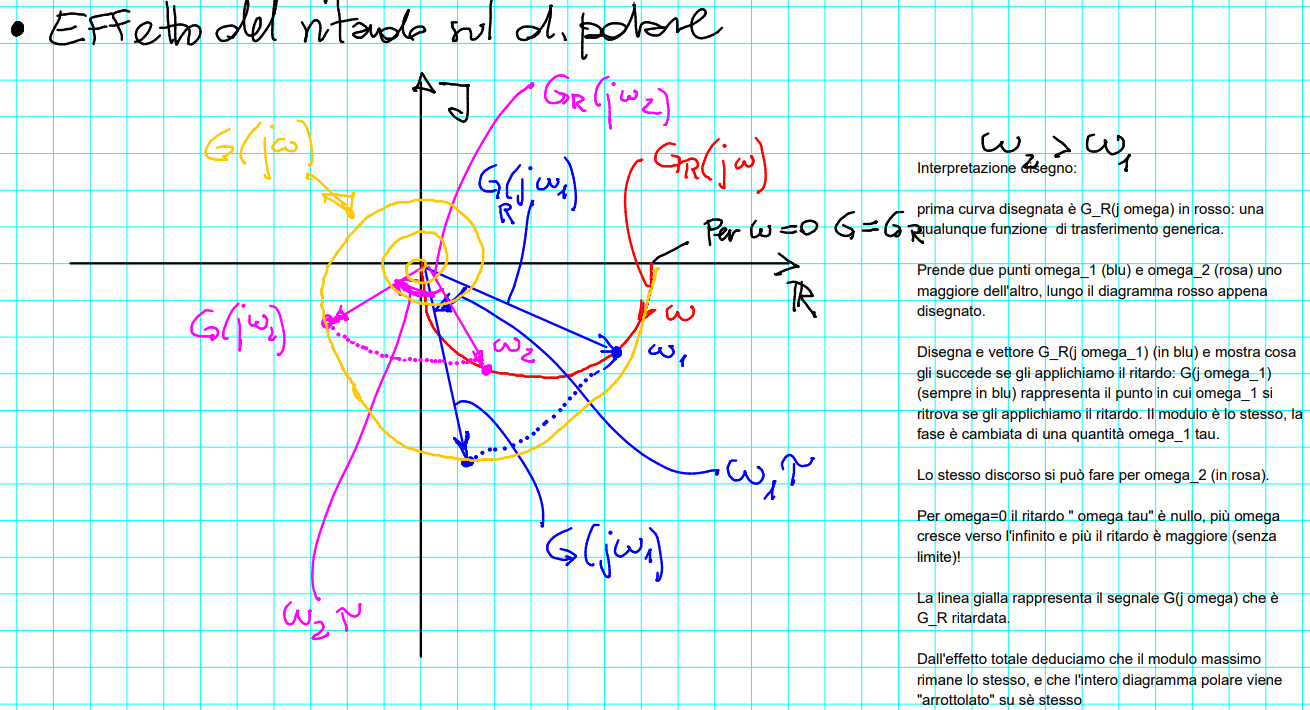
\includegraphics[height=3cm]{../lezione17/img2.PNG}
        \end{center}
        Data $G = \frac{N}{D} e^{- j \omega \tau}$ ci sono due casi possibili:
        \begin{itemize}
            \item Caso in cui il grado di $D$ sia maggiore del grado di $N$: il diagramma polare di $G$ dinisce nell'origine con fase tendente a $- \infty$, quindi il diagramma si arrotola su sè stesso come una spirale;
            \item Caso in cui il grado di $D$ sia uguale al grado di $N$: il modulo è costante e la fase tende a $- \infty$, quindi il diagramma diventa una circonferenza percorsa infinite volte.
        \end{itemize}
\end{multicols*}
\begin{multicols*}{2}
    \newpage\section{Funzioni fondamentali di un anello di controllo}
    \begin{itemize}
        \item funzione di traferimento d'anello (aperto) $L(s) := R(s) \cdot P(s)$;
        \item funzione di sensitività complementare $T(s) := \frac{L(s)}{1+ L(s)}$;
        \item funzione di sensitività $S(s) := \frac{1}{1+ L(s)}$;
        \item funzione di sensitività del controllo $Q(s) := \frac{R(s)}{1+L(s)}$
        \item $\frac{Y}{W} = \frac{L}{1+L} = T$;
        \item $\frac{Y}{D_r} = - \frac{L}{1+L} = -T$;
        \item $\frac{Y}{D_a} = \frac{1}{1+L} = S$;
        \item $Y = T \cdot W + S \cdot  D_a -T \cdot D_r = T \cdot W + S \cdot D_a - T \cdot D_r$.
    \end{itemize}
    \section{Stabilità di sistemi retroazionati}
    \subsection{Diagramma di Nyquist}
    \textbf{Percorso di Nyquist}: Curva chiusa costituita dall'intero asse immaginario e da una semicirconferenza di raggio infinito giacente nel semipiano destro. Se $G(s)$ ha poli a parte reale nulla, il percorso di Nyquist viene modificato evitando tali poli con semicirconferenze di raggio infinitesimo giacenti nel semipiano destro. Il percorso di Nyquist è percorso in senso antiorario.\newline
    \newline
    \textbf{Diagramma di Nyquist}: Costituito dal diagramma polare e della sua immagine speculare rispetto all'asse reale.
    \subsection{Stabilità asintotica}
    \begin{itemize}
        \item Il numero di giri antiorari del diagramma di Nyquist di $G(s)$ attorno all'oigine è \textbf{uguale} al numero di poli di $G(s)$ circondati dal suo percorso di Nyquist in senso orario \textbf{meno} il numero di zeri di $G(s)$ circondati dal suo percorso di Nyquist in senso orario.
        \item Detto $L(s) = R(s) \cdot P(s)$, allora:\newline
        il numero di giri del diagramma di Nyquist di $L(s)$ attorno al punto $-1$ è \textbf{uguale} al numero di poli di $L(s)$ con $Re> 0$ \textbf{meno} il numero di poli dell'anello chiuso con $Re > 0$.
    \end{itemize}
    Poichè per avere la \textbf{stabilità asintotica} dell'anello chiuso si vuole che il numero di poli dell'anello chiuso con $Re > 0$ sia uguale a zero, si ha che deve essere:\newline
    numero di iri del diagramma di Nyquist di $L(s)$ attorno al punto $-1$ è \textbf{uguale} al numero di poli di $L(s)$ con $Re > 0$.
    \subsection{Criterio di Nyquist}
    Considerando il sistema dinamico:
    \begin{center}
        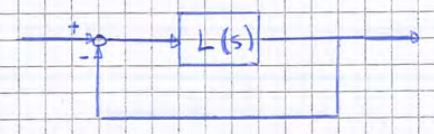
\includegraphics[height=1cm]{../formulario/img1.JPG}
    \end{center}
    \begin{itemize}
        \item Si tracci il diagramma di Nyquist di $L(s)$;
        \item Sia $P_D$ il numero di poli di $L(s)$ con $Re > 0$;
        \item Sia $N$ il numero di giri antiorari del diagramma di Nyquist di $L(s)$ attorno al punto $-1$ dell'asse reale; se il diagramma di Nyquist passa per il punto $-1$ si dirà che $N$ non è ben definito.
    \end{itemize}
    \textbf{Criterio}: il sistema in anello chiuso è asintoticamente stabile $\Leftrightarrow$ $N$ è ben definito e $N = P_D$.
    \begin{itemize}
        \item \textbf{Caso $N$ non ben definito}:\newline
        se $N$ non è ben definito, allora il diagramma di Nyquist passa per $-1$, il sistema in anello chiuso ha poli con parte reale nulla, quindi è \textbf{non asintoticamnete stabile} (stabile o instabile, ma non si può concludere nulla a proposito).\newline
        \item \textbf{Caso $N \neq P_D$}:\newline
        Se $N$ è ben definito ma $N\neq P_D$, il sistema in anello chiuso è sicuramento \textbf{instabile}.\newline
        \item \textbf{Caso particolare $P_D = 0$}:\newline
        In questo caso per essere asintoticamente stabile deve essere $N = 0$. Si possono in questo caso definire dei margini di stabilità:
        \begin{itemize}
            \item Margine di modulo: $M_m = min_{\omega} | 1 + L(j \omega)|$;
            \item Margine di guadagno: $K_m = \frac{1}{\alpha}$, dove $\alpha$ è il valore del modulo nel punto in cui interseca l'asse dei reali negativi ($\mathbb{R}^{-}$);
            \item Margine di fase: $\omega_c$: frequenza tache che $|L| = 1$, $\phi_c = arg(L(j \omega_c))$, $\phi_m = -180 - |\phi_c|$.
        \end{itemize}
    \end{itemize}
    \subsection{Criterio di Bode}
    \begin{itemize}
        \item Sia $P_D = 0$ (cioè $L(s)$ non ha poli con $Re > 0$);
        \item Sia il diagramma di Bode del modulo di $L(s)$ tale che intersechi l'asse $0_{dB}$ una sola volta dall'alto verso il basso (cioè $L$ entra una sola volta nele cerchio unitario e non ne esce più);
        \item Sia $\mu_L$ il guadagno di $L(s)$ e $\phi_m$ il margine di fase;
    \end{itemize}
    Allora il sistema in anello chiuso è asintoticamente stabile se e solo se ($\Leftrightarrow$) $\mu_L > 0$ e $\phi_m > 0^o$
    \newpage\section{Sintesi del controllore in retroazione}
    SD LTI A TC SISO nell'ipotesi di Bode.
    \begin{center}
        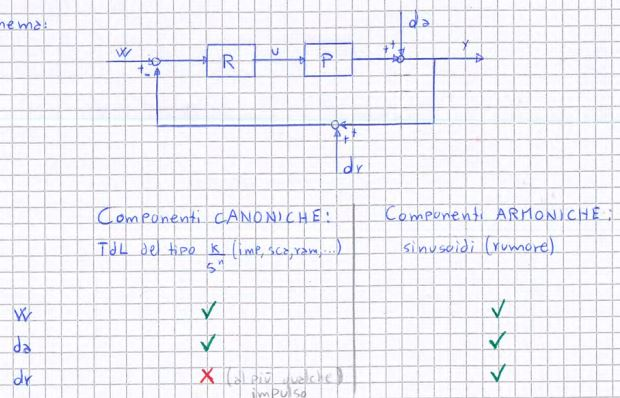
\includegraphics[height=3cm]{../formulario/img2.JPG}
    \end{center}
    \subsection{Progetto statico}
    \begin{itemize}
        \item assumo che il sistema AC sia AS.
        \item Considero le sole componenti canoniche $w$ e $d_a$
        \item Calcolo l'errore a transitorio esaurito con il teorema del valore finale:\newline
        $e_\infty = \lim_{t\rightarrow +\infty} e(t)$ dove $e(t) : = w(t) - y(t)$.\newline
        Vediamo i conti da fare:
        \begin{itemize}
            \item caso di influenza di $w$: si indica con $\frac{E}{W}$ la funzione di trasferimento da $W$ a $E$; $e_\infty = \lim_{s\rightarrow 0} s \cdot W(s) \cdot \frac{E(s)}{W(s)} = s \cdot W \cdot  \frac{1}{1+L} = \lim_{s\rightarrow 0} s \cdot W \cdot \frac{1}{1+ \frac{\mu_L}{s^{g_L}} \cdot \frac{1 + \dots}{1 + \dots}}$, dove $\frac{1 + \dots}{1 + \dots}$ va a $1$ per $s \rightarrow 0$, da cui ottengo che $\lim_{s\rightarrow 0} s \cdot W \cdot \frac{s^{g_L}}{s^{g_L} + \mu_L}$.
            \item caso di influenza di $d_a$: in questo caso si usa $\frac{E}{D_a} = - \frac{1}{1+L}$, e quindi: $e_\infty = \lim_{s\rightarrow 0} s \cdot D_a(s) \cdot \frac{E(s)}{D_a(s)}$
        \end{itemize}
        infine si sceglie il vincolo più restrittivo tra quello per $w$ e quello per $d_a$.
        \item Impongo i vincoli ($e_\infty = 0$ oppure $|e_\infty| < $ un certo valore), e determino condizioni su tipo e/o guadagno di $L(s)$, ricordando che si cerca di avere sempre $g_L$ il minimo necessario e che per le condizioni di Bode si deve avere $\mu_L > 0$.
    \end{itemize}
    In generale, ponendo: \newline
    $P(s) = \frac{\mu_p}{s^{g_p} \cdot  \frac{1+ \dots}{1+ \dots}}$;\newline
    $R(s) = \frac{\mu_r}{s^{g_r}} \cdot  \frac{1+ \dots}{1+ \dots}$;\newline
    Si ottiene: \newline
    $L(s) = R(s) \cdot P(s) \rightarrow \begin{cases}
        \mu_L = \mu_r \cdot \mu_p\\
        g_L = g_r + g_p
    \end{cases}$\newline
    Ricordiamo che:\newline
    $\frac{Y}{W} = - \frac{Y}{D_r} = \frac{L}{1+L} = T$\newline
    $\frac{Y}{D_a} = \frac{1}{1+L} = S$
    \subsection{Progetto dinamico}
    \begin{center}
        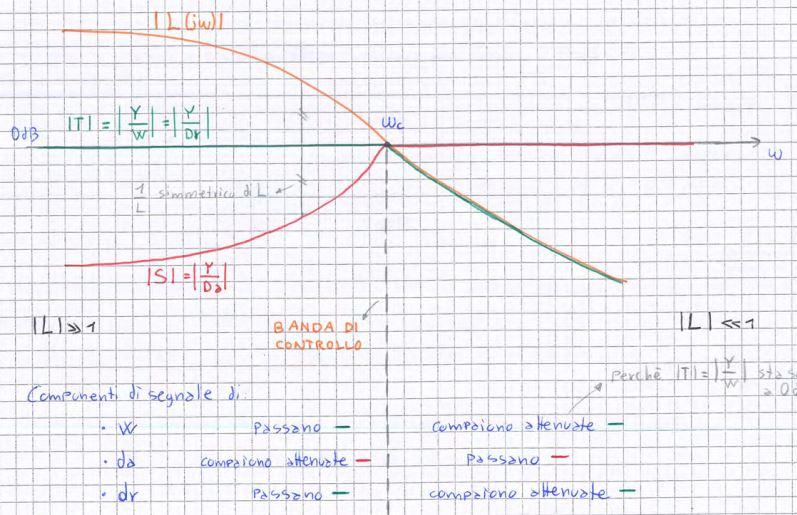
\includegraphics[height=3cm]{../formulario/img3.JPG}
    \end{center}
    $T = \frac{Y}{W} = - \frac{y}{D_r}\; \text{componente di $Y$ dovuto a $W$}\; = \frac{L}{1+L} = \begin{cases}
        1 \; \text{se}\; |L| >> 1\\
        L \; \text{se}\; |L| << 1
    \end{cases}$\newline
    $S = \frac{Y}{D_a} =\; \text{componente di $Y$ dovuto a $D_a$}\; = \frac{1}{1+L} = \begin{cases}
        \frac{1}{L} \; \text{se}\; |L| >> 1\\
        1 \; \text{se}\; |L| << 1
    \end{cases}$\newline
    \newline
    \textbf{Vincolo sulla velocità di risposta}: ($\omega_c$ è la frequenza critica, cioè dove $L$ interseca l'asse $0_{dB}$) $\omega_{c_{min}} < \omega_c < \omega_{c_{max}}$, quindi $|L(j \omega)|$ deve tagliare l'asse $0_{dB}$ entro i limiti posti a $\omega_c$. \newline
    nota bene: si cerca inizia sempre la costruzione di $L(s)$ a partire da un tratto con pendenza $-1$ il più lungo possibile (così avremo il vantaggio di avere un margine di fase maggiore).\newline
    \textbf{Vincolo sul grado di stabilità (e assenza di oscillazioni)}: $\phi_m > $ un determinato valore (si verifica con il regolo delle fasi). In caso di $P(s)$ con ritardo, allora ricordarsi di tenerne conto nel calcolo della fase critica (che serve per il calcolo del margine di fase) con la solita formula $-\omega_c \tau$.\newline
    \textbf{Vincolo sulla reiezione di un disturbo in andata}: un disturbo sinusoidale (le componenti canoniche sono state gestite nel progetto statico) $d_a(t) = A sin (\omega_a \cdot  t)$ con $|A| < \bar{A}$ e $0 \leq \omega_{a_1} \leq \omega_a \leq \omega_{a_2} \leq \omega_c$, deve produrre asintoticamnete (per $t \rightarrow \infty$) su $y$ un effetto di ampiezza non superiore a $\Delta_a$ (ampiezza del massimo effetto che tollero).\newline
    Per rispettare il vincolo occorre che nella banda su cui insiste il disturbo (da $\omega_{a1}$ a $\omega_{a2}$), il modulo della funzione di trasferimento dal disturbo $d_a$ all'uscita $y$ sia più picolo di $\frac{\text{"max ampiezza accettabile dell'effetto su y}}{\text{max ampiezza possibile del disturbo}}$.\newline
    In definitiva bisogna che:
    \[
        |L(j \omega)| > \frac{\bar{A}}{\Delta a} \;\;\;\text{per}\; \omega_{a_1} \leq \omega \leq \omega_{a_2}
    \]
    \begin{center}
        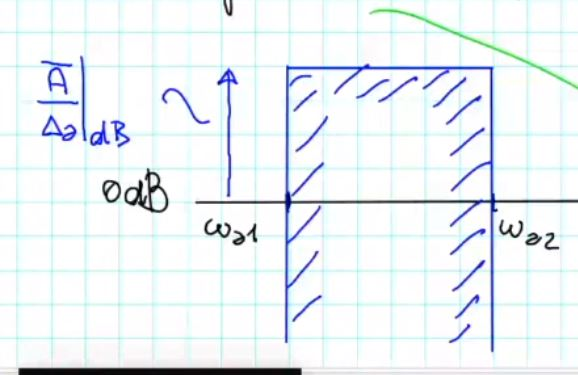
\includegraphics[height=2cm]{../formulario/img8.JPG}
    \end{center}
    \textbf{Vincolo sulla reiezione di un disturbo in retroazione}: un disturbo sinusoidale $d_r(t) = B \cdot  sin(\omega_r \cdot t)$ con $|b| < \bar{B}$ e $\omega_c < \omega_{r_1} \leq \omega_r \leq \omega_{r_2} \leq \infty$, deve produrre asintoticamente (per $t \rightarrow  \infty$) su $y$ un effetto di ampiezza non superiore a $\Delta r$. In definitiva bisogna che:
    \[
        |L(j \omega)| < \frac{\Delta r }{\bar{B}} \;\;\;\text{per}\; \omega_{r_1} \leq \omega \leq \omega_{r_2}
    \]
    \begin{center}
        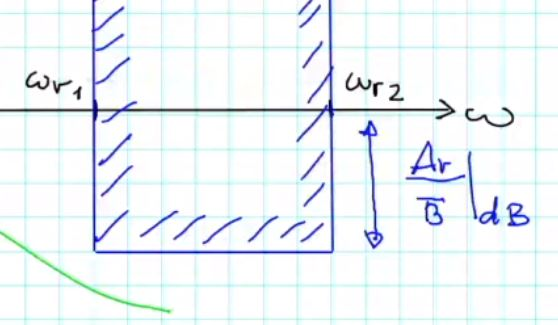
\includegraphics[height=2cm]{../formulario/img9.JPG}
    \end{center}
    \rule{\textwidth}{0,4pt}
    In conclusione occorre trovare "per tentativi" una funzione di trasferimento $L(s)$ che:
    \begin{itemize}
        \item se $P(s)$ ha un ritardo, anche nella formula finale di $L(s)$ sarà presente (!!);
        \item rispetti i vincoli del progetto statico;
        \item rispetti i vincoli del progetto statico;
        \item contenga eventuali zeri di $P(s)$ nel semipiano destro ($R(s)$ non li cancelli): \textbf{no cancellazioni nel semipiano destro!}. $P(s)$ è solitamente un dato del problema, dunque si controlla subito se ci sono zeri nel semipiano destro, se ci sono, sappiamo che di sicuro li avremo anche in $L(s)$, e di conseguenza dobbiamo costruirlo tenendolo in mente.
        \item produca un margine di fase $\phi_m$ adeguato;
        \item abbiamo un grado relativo almeno pari a quello di $P(s)$ (altrimenti $R(s)$ viene con più zeri che poli);
        \item abbia meno zeri e poli possibile.
    \end{itemize}
    Fatto ciò si trova $R(s) = \frac{L(s)}{P(s)}$.\newline
    \subsection{Sistema dinamico (AS) "a fase minima"}
    Un SD LTI a TC AS è a fase minima se:
    \begin{itemize}
        \item no zeri nel semipiano destro;
        \item no ritardi
    \end{itemize}
    Se un sistema è a fase minima, il DBF si può dedurre dalla conoscenza del DBM e del segno del guadagno, perchè tutti i poli/zeri sono nel semipiano sinistro e non ci sono ritardi, quindi, DBF inizia da $0^o$ se $\mu> 0$ o da $-180^o$ se $\mu< 0$, e poi un polo è $-90^o$ e uno zero è $+ 90^o$.\newline
    Inoltre, se un SD a fase minima e con $mu > 0$ ha il DBM con un lungo tratto a pendenza $-1$, allora nella parte centrale di quel tratto, la sua fase è circa $-90^o$, questo motiva il "tratto lungo a pendenza $-1$ attorno a $\omega_c$".\newline
    Anche nel caso non a fase minima rimane una buona idea, purchè gli zeri a destra siano a $\omega > \omega_c$ e il contributo si eventuali ritardi non sia eccessivo.
    \section{compensazione di un disturbo misurabile}
    Se $d$ ha componenti così veloci che la retroazione non può contrastarle e non è possibile/opportuno aumentare $\omega_c$, allora faccio la compensazione. \newline
    La compensazione serve se $\omega_d \leq \omega_c$, ma in realtà anche solo se sono vicini.
    \begin{center}
        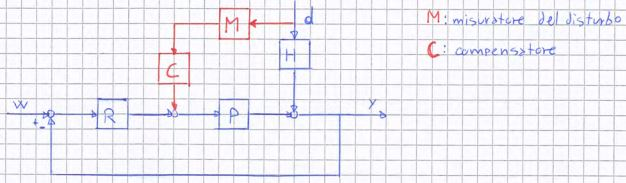
\includegraphics[height=2cm]{../formulario/img4.JPG}
    \end{center}
    $C_{ID}: \frac{Y}{D} = 0 \Rightarrow \frac{Y}{D} = \frac{H + MCD}{1+RP} = 0 \Rightarrow H + MCP = 0 \Rightarrow C_{ID} = - \frac{H}{MP}$.\newline
    Tuttavia $C_{ID}$ può non essere realizzabile se:
    \begin{itemize}
        \item $C_{ID}$ ha più zeri che poli (non realizzabile);
        \item $C_{ID}$ è instabile: $H$ è AS per definizione (essendo fuori anello, deve esserlo), ma $P$ può avere zeri nel semipiano destro.
    \end{itemize} 
    Se $C_{ID}$ non si può implementare, occore conoscere un limite superiore $\omega_d$ per la banda del disturbo (cioè $d$ non ha componenti di segnale per $\omega > \omega_d$) e trovare una funzione di trasferimento $C(s)$ reale realizzabile (aggiungere poli o togliere zeri per rendere realizzabile il controllore, solitamente dopo due decadi da $\omega_d$) e AS tale che $C(j \omega) \sim C_{ID} (j \omega)$ per $\omega \leq \omega_d$ in modulo e fase.\newline
    \newline
    A livello pratico: si cerca di ottenere un $L(s) = \frac{\omega_c}{s}$ (o almeno è approssimabile così nei pressi di $\omega_c$), da qui si trova $R(s)$. Calcoliamo ora $C_{ID} = - \frac{H}{MP}$ e guardiamo se è realizzabile. Se lo è siamo a posto, se non lo è: tracciamo il diagramma di Bode del modulo di $C_{ID}$ e ci sengamo la banda del disturbo (che arriva fino a $\omega_d$) e andiamo avanti di due decadi da $\omega_d$. Da qui si possono aggiungere poli e/o togliere zeri per costruire un $C_{RE}$ realizzabile.
    \section{Controllo a due gradi di libertà}
    \begin{center}
        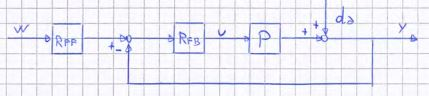
\includegraphics[height=2cm]{../formulario/img5.JPG}
    \end{center}
    $\frac{Y}{D_a} = \frac{1}{1+R_{FB} \cdot P}$\newline
    $\frac{Y}{W} = \frac{R_{FF} R_{FB} P}{1 + R_{FB} P}$
    \section{Cenno al progetto del regolatore in condizioni d'incertezza}
    Cosa succede se il modello $P(s)$ non è una descrizione esatta del processo?\newline
    Per esempio se $P(s) = P_n(s) + \Delta P(s)$, dove $P_n(s)$ è l'unico elemento a noi noto e sappiamo $|\Delta P(j \omega)| < f(\omega)$ con $f(\omega)$ nota. \newline
    Siamo in ipotesi di Bode e in particolare $P_n$ non ha poli con $Re > 0$ e nemmeno $P_n + \Delta P$.\newline
    Il sistema nominale (AC con $P_n$ e il regolatore $R$ progettato su $P_n$) è AS.\newline
    Voglio trovare condizioni su $|\Delta P (j \omega)|$ che garantiscano la stabilità asintotica dell'anello chiuso in sua presenza.\newline
    Una condizione sufficiente per la robustezza dell'AS dell'AC a fronte di perturbazioni di modello additive è $|R \Delta P| < |1 + L_n|$ e $|\Delta P| < | \frac{1 + L_n}{R}| = | \frac{1}{Q_n}|$.\newline
    Allora se possiedo una $f(\omega)$ progetterò $R(s)$ in modo che $f(\omega) < | \frac{1}{Q_n}| $ per ogni $\omega$.
    \newpage\section{Regolatore PID}
    Legge di controllo ideale :
    \[
        u(t) = u_P + u_I + u_D = k_P \cdot e(t) + k_I \cdot \int_{0}^{t}e(\tau)d \tau + k_D \cdot \frac{d e (t)}{dt}
    \]
    \subsection{Azione proporzionale P}
    Ruolo: garantire una risposta pronta a reiezioni dell'errore. \newline
    \newline
    $u_P = k_P \cdot e \rightarrow $ "più errore, più azione di controllo".\newline
    Se $u$ è soltanto $u_P$, abbiamo $u \neq 0 \Leftrightarrow e \neq 0$ (male).\newline
    Se $u$ non è soltanto $u_P$, abbiamo $u = u_P + \bar{u}$ e quindi scegliamo $\bar{u}$ in modo tale che $e = 0$, da notare che $\bar{u}$ dipende dal set point (il valore desiderato $w$).\newline
    Per calcolare $\bar{u}$, supponiamo $\mu_P > 0$, otteniamo che se $e= 0$, ho già trovato quello che cerco, se $e<0$ allora deve crescere, se $e>0$ allora deve decrescere. Notiamo quindi che $\bar{u}$ è proporzionale all'integrale dell'errore $\int e dt$.
    \subsection{Azione integrale I}
    Ruolo: garantire errore nullo a regime. \newline
    \newline
    $u_I = k_I \cdot \int_{0}^{t} e (tau) d \tau$, se il sistema in AC va a regime (costante), allora in presenza di azioni $I$ l'errore è nullo.
    \subsection{Azione derivativa D}
    Ruolo: "anticipare" l'errore.\newline
    \newline
    $\tilde{e}(\bar{t} + T_d) = e(\bar{t}) + \frac{d e(t)}{dt}_{t= \bar{t}} \cdot T_d$, dove il termine $\frac{d e(t)}{dt}_{t= \bar{t}} \cdot T_d$ è la variazione prevista di $e(t)$ sull'orizzonte $T_d$.\newline
    \newline
    $u_D =  k_D \cdot \frac{d e (t)}{dt}$ è proporzionale alla variazione prevista dell'errore: $T_d$ è l'orizzonte di questa predizione e K è il fattore di proporzionalità.
    \subsection{Forme alternative della legge di controllo PID}
    \begin{itemize}
        \item vediamo $u$ trasformata secondo Laplace in forma ISA IDEALE (2 zeri e 1 polo):
        \[
            U = (k_P + \frac{k_I}{s} + k_D \cdot s) E = K ( 1 + \frac{1}{sT_i} + s T_d) \cdot E = K \left( \frac{sT_i + 1 + s^2 T_i T_d}{sT_i} \right) \cdot E
        \]
        con $K = k_P$ "guadagno", $k_I = \frac{k_P}{T_i}$, $k_D = k_P T_D$, $T_i$ tempo integrale e $T_d$ tempo derivato.
        \item Forma ISA reale a un grado di libertà:
        \[
            U = K \left( 1+ \frac{1}{sT_i} + \frac{sT_d}{1+s \frac{T_d}{N}}\right)
        \]
        \item Forma ISA reale a due gradi di libertà:
        \[
            U = K \left( b W - Y + \frac{1}{sT_i}(W-Y) + \frac{sT_d}{1+s \frac{T_d}{N}} (c W-Y)\right)
        \]
        con $b$ pesi del set point nelle azioni P, e $c$ pesi del set point nelle azioni $D$. 
    \end{itemize}
    Riassumendo:
    \begin{itemize}
        \item PID: regolatore con 2 zeri e 2 poli (di cui uno nell'origine): $\mu \cdot \frac{(1+sT_1) (1+sT_2)}{s(1+s \tau)}$;
        \item PI: regolatore con 1 zero e 1 polo (nell'origine): $\mu \cdot  \frac{1+sT}{s} = \mu(\frac{1}{s}+ T)$ 
    \end{itemize} 
    \subsection{Metodi di taratura}
    \textbf{modello}: $\mu, T_1, T_2$.\newline
    \textbf{specifiche}: $\bar{\omega}_c, \bar{\phi}_m$.\newline
    \newline
    Dato un $P(s) = \frac{\mu}{(1+sT_1) (1+sT_2)}$ uso le seguenti equazioni per la taratura dei parametri del PID nella forma $R(s) = \mu_R \frac{(1+sT_{R1}) (1+sT_{R2})}{S (1+s \tau_R)}$:
    \begin{itemize}
        \item poniamo $T_{R1} = T_1$ e $T_{R2} = T_2$ e ottengo un $L(s) = \frac{\mu \mu_R}{s(1+s \tau_R)}$.
        \item $\bar{\omega}_c$: $\mu \cdot \mu_R = \bar{\omega}_c \rightarrow \mu_R = \frac{\bar{\omega}_c}{\mu}$;
        \item $\bar{\phi}_m$: $90^o - arctg^o(\mu \mu_R \tau_R) = \bar{\phi}_m \rightarrow \tau_R = \frac{1}{\mu \mu_R} tg(90^o - \bar{\phi}_m)$  
    \end{itemize}
    Vediamo ora due metodi di traratura: "IMG PID tuning per processi AS" e "Metodo di Ziegler-Nichols".
    \subsection{Principio del modello interno (IMC)}
    \begin{center}
        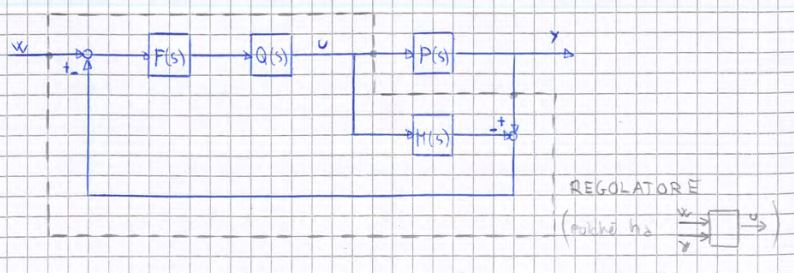
\includegraphics[height=2cm]{../formulario/img6.JPG}
    \end{center}
    \begin{itemize}
        \item In condizioni nominali (cioè: $M(s) = P(s)$, modello esatto, no incertezza, nessun disturbo) l'anello è aperto ( segnale di retroazione è identiamente nullo);
        \item $Y(s) = F(s)Q(s)P(s)W(s) = F(s) Q(s)M(s)W(s)$;
        \item se si può porre $Q(s) = \frac{1}{M(s)}$, allora $Y(s) = F(s) W(s)$, per cui si può scegliere $F(s)$ "ad arbitrio", purchè $FQ$ sia realizzabile
    \end{itemize}
    \subsection{Regola di taratura per IMG PID per processi AS}
    assumiamo $P(s) = \mu \frac{e^{-s \tau}}{1+s T}$ con $T> 0$ (AS), $\tau \geq 0$ e $\mu > 0$ per comodità.\newline
    \newline
    Ora creiamo $Q$ e $F$:
    \begin{itemize}
        \item $Q(s) = \frac{1 + s T}{\mu}$: inverto quel che posso di $P(s)$, ovvero la parte a fase minima, ma non il ritardo.
        \item $F(s) = \frac{1}{1+s \lambda}$: almeno un polo sennò $QF$ non è realizzabile e $\lambda$ è solo il nome di una costante di tempo, come "$T$".
    \end{itemize}
    $R(s)$ ha la forma: $R(s)= \frac{Q(s) F(s)}{1- Q(s)F(s)M(s)}$. Sostituendo i termini trovati prima otteniamo
    \[
        R = \frac{1}{\mu} \cdot \frac{1+sT}{1+s \lambda - e^{-s \tau}}
    \]
    quindi dobbiamo approssimare $e^{-s \tau}$ con una funzione di trasferimento razionale fratta, per farlo usiamo gli \textbf{approssimanti di Padè} (Padè$(z,p)$, con $p$ poli e $z$ zeri):
    \begin{itemize}
        \item Padè $(1,0) = 1- s \tau$: otteniamo un PI con $R(S) = \frac{1}{\mu} \frac{1+sT}{s(\lambda + \tau)}$, che può essere visto anche nella forma $R(s) = k \frac{1+ s T_i}{sT_i}$ con $T_i = T$ e $\frac{k}{T_i} = \frac{1}{\mu(\lambda+\tau)}$ e $k = \frac{T}{\mu(\lambda + \tau)}$.
        \item Padè $(1,1) = \frac{1-s \tau/2}{1 + s \tau/2}$: otteniamo un PID reale con $R(s) = \frac{1}{\mu (\lambda + \tau)} \frac{(1+sT) (1+s \tau/2)}{s (1+ s \frac{\lambda \tau}{s (\lambda + \tau)})}$
    \end{itemize}
    \subsection{Metodo di Ziegler-Nichols}
    In anello chiuso:
    \begin{itemize}
        \item si chiuse l'anello di controllo con il regolatore PID (i cui parametri devono essere sintetizzati), imponendo nulle leazioni integrale e derivata, cioè $k_I = 0$, $k_D = 0$.
        \item Partendo da valori molto piccoli di $k_P$ si effettua un semplice esperimento, consistente nell'applicare un piccolo gradino al segnale di riferimento.
        \item Si aumenta progressivamente $k_P$ ripetendo di volta in volta l'esperimento finchè non si instaura nell'anello un'oscillazione permanente.
        \item Detto $\bar{k}_P$ il valore del guadagno proporzionale corrispondente all'oscillazione permanente (guadagno critico) e $\bar{T}$ il periodo di tale oscillazione, si tarano i parametri di un regolatore $P, PI$ o $PID$ sulla base della seguente tabella:
        \begin{center}
            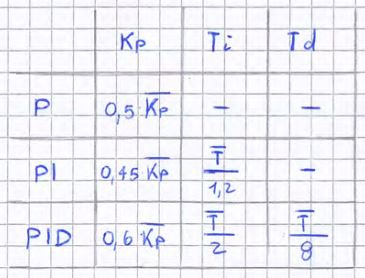
\includegraphics[height=3cm]{../formulario/img7.JPG}
        \end{center}
    \end{itemize}
    \subsection{PID a due gradi di libertà ed effetto dei pesi b e c e di N sugli zeri}
    Dalla formula ISA:\newline
    $U = R_1 - R_2 =  k \left( b + \frac{1}{sT_i} + \frac{c s T_d}{1 + s \frac{T_d}{N}} \right) W - k\left( 1 + \frac{1}{sT_i} + \frac{sT_d}{1 + s \frac{T_d}{N}} \right)Y$ \newline
    con \newline
    $R_1 = k \left( b + \frac{1}{sT_i} + \frac{c s T_d}{1 + s \frac{T_d}{N}} \right) W$\newline
    $R_2 = k\left( 1 + \frac{1}{sT_i} + \frac{sT_d}{1 + s \frac{T_d}{N}} \right)Y$\newline
    \newline
    Il problema sono gli $\frac{1}{s}$ nei termini $R_1$ e $R_2$, che rendono il blocco non AS, quindi non si possono realizzare così.\newline
    \newline
    Per risolvere il problema :\newline
    $R_{FB} = R_2 =  K \frac{1 + s\left(T_i + \frac{T_d}{N}\right) + s^2 T_i T_d \left(1 + \frac{1}{N}\right)}{sT_i \left( 1 + \frac{sT_d}{N}\right)}$.\newline
    $R_{FF} = \frac{R_1}{R_2} =  \frac{1+ s\left(bT_i + \frac{T_d}{N}\right) + s^2 T_i T_d \left(c + \frac{b}{N}\right)}{1 + s \left( T_i + \frac{T_d}{N} \right) + s^2 T_i T_d \left( 1 + \frac{1}{N} \right)}$
    \section{Cenno al controllo di sistemi instabili}
    Vedremo 2 casi:
    \begin{itemize}
        \item Sistema del prim'ordine con un polo instabile: es. $P(S) = \frac{\mu}{1-s \tau}$.\newline
        Chiuso un primo anello attorno a P col solo scopo di ottenre che tale anello (chiuso) sia AS.\newline
        polo: $1-s T + k \mu = 0$, $S_{polo} = \frac{1 + k \mu}{T}$, scelgo un qualunque $k$ tale da rendere $S_{polo} < 0$. Ora chiudo un secondo anello attorno al primo ponendomi nelle ipotesi di Bode. Ottengo $R_2$ in modo da avere $\omega_c, \phi_m, \dots$ coi metodi noti.
        \item Sistema del second'ordine con un polo instabile: es. consideriamo due casi $P_1(s) = \frac{1}{(1+s) (1-5s)}$, $P_2(s) = \frac{1}{(1+5s) ( 1-s)}$.\newline
        \begin{itemize}
            \item per $P_1$: $R_1 = k \Rightarrow L = \frac{k}{(1+s) (1-5s)}$; $\frac{R_1 P_1}{1+R-1P_1} =  \frac{L}{1+L} = \frac{k}{1-4s-5s^2 + k}$, in cui il denominatore ha poli con $Re<0$ se $k+1<0$. Da qui sappiamo cosa fare (vedi caso precedente).
            \item per $P_2$: $R_1 = k \Rightarrow L = \frac{k}{(1+5s) (1-s)}$; $\frac{R_1 P_2}{1+ R_1 P_2} = \frac{k}{-5s^2 + 4s \dots}$, ci fermiamo perchè non esiste $k$ che lo renda AS. Però il polo sinistro si può cancellare e quindi con $R_1$ fatto da un polo e uno zero ci si può ripostare al caso $P_1$. Nell'esempio si ottiene $R_1(s) = k \frac{1+5s}{1+0,5 s}$ e otteniamo $L = \frac{k}{(1+0,5 s) (1-s)}$ che rimanda al caso $P_1$. 
        \end{itemize}
    \end{itemize}
    \newpage\section{Sistemi di controllo digitale}
    \subsection{Trasformata Zeta}
    Dato un segnale (reale) a TD $v(k)$, si definisce la sua trasformata Zeta $V(z) = \mathcal{Z}[v(k)] := \sum_{k=0}^{\infty} v(k) z^{-k}$, con $z$ e $V(z)$ complessi.\newline
    \textbf{Proprietà}:
    \begin{itemize}
        \item La trasformata di Zeta è un operatore lineare;
        \item Trasformata di Zeta anticipata di un passo: $\mathcal{Z}[v(k+1)] = \sum_{k=0}^{\infty} v(k+1) z^{-k} = z \mathcal{Z}[v(k)] - z v(0)$;
    \end{itemize}
    \textbf{Trasformate Zeta notevoli}:
    \begin{itemize}
        \item impulso: $\mathcal{Z}[imp(k)] = 1$
        \item scalino: $\mathcal{Z}[sca(k)] = \frac{z}{z-1}$ per $|z|>1$
        \item esponenziale: $\mathcal{Z}[a^k sca(k)] = \frac{z}{z-a}$ per $|z| > |a|$
    \end{itemize}
    \subsubsection{Funzione di trasferimento}
    \textbf{Trasformata Zeta dell'equazione di stato}:
    \[
        X(z) = (zI-A)^{-1} z x(0) + (zI-A)^{-1} b U(z)
    \]
    \textbf{Trasformata Zeta dell'equazione d'uscita}:
    \[
        Y(z) = cX(z) + dU(z) = c(zI-A)^{-1} z x(0) + [c(zI-A)^{-1} b + d] U(z)
    \]
    \textbf{Funzione di trasferimento}:
    \[
        c(zI-A)^{-1} b + d
    \]
    Siccome la funzione di trasferimento è uguale a quello di SD a TC, posso fare le stesse considerazioni su stabilità, poli, autovalori, parti nascoste, raggiungibilità, osservabilità.\newline
    \newline
    \textbf{Schema a blocchi}:\newline
    Per la stesura dello schema a blocchi si può usare il metodo degli integratori $\frac{1}{s}$ a TC, ma con un blocco $z^{-1}$:
    \begin{center}
        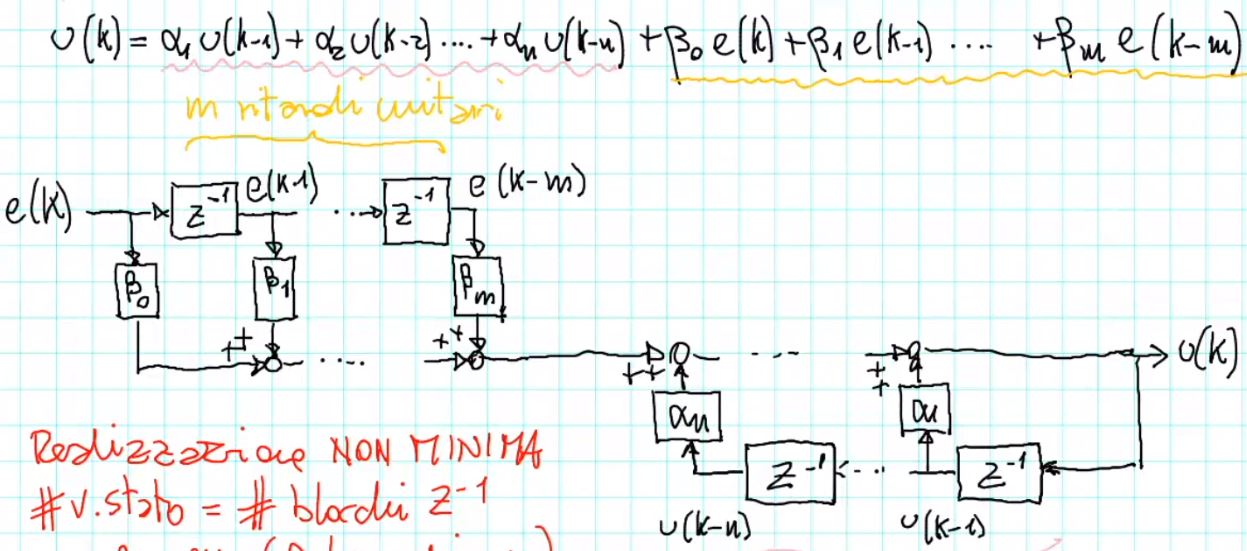
\includegraphics[height=5cm]{../formulario/img14.JPG}
    \end{center} 
    Per quanto riguarda i paralleli/le serie/ gli anelli le formule sono le medesime a TC. 
    \subsection{Schema di controllo (loop) ibrido}
    \begin{center}
        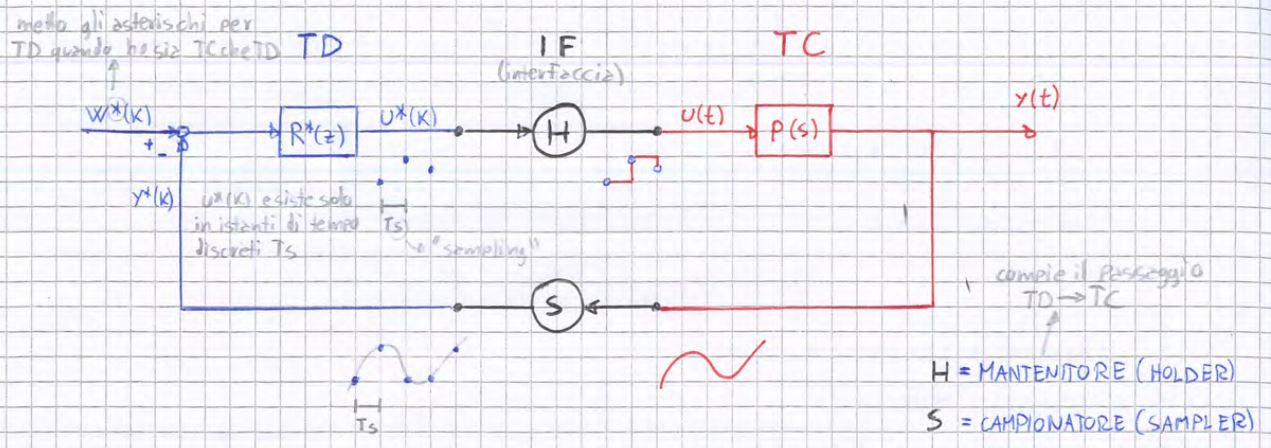
\includegraphics[height=3cm]{../formulario/img10.JPG}
    \end{center}
    In questo corso consideriamo:
    \begin{itemize}
        \item campionatore (sampler) idele: $y^*(k) = y(k T_s)$
        \item mantenitore (holder) di ordine zero (ZOH): $u(t) = u^*(k)$ per $k T_s \leq t < (k+1)T_s$
    \end{itemize}
    \textbf{problema}: noi progettiamo il regolatore $R(s)$ nello schema solito, ovvero come se fosse tutto a TC, poi però dobbiamo ottenere $R^*(z)$ e implementare lo schema SH (sampling and holding) dovendo anche scegliere il tempo di campionamneto $T_s$.\newline
    Dividiamo il problema in:
    \begin{itemize}
        \item scelta di $T_s$ (tempo di campionamento);
        \item discretizzazione: $\{R(s), T_s\} \rightarrow  R^*(z)$;
    \end{itemize}
    \subsection{Scelta di $T_s$}
    Problema: abbiamo un segnale $f(t)$ che facciamo entrare in un campionatore e otteniamo un segnale $f^{\#}(t)$ o $f^*(k)$, che a sua volta entra in un ZOH e otteniamo un segnale $y(t)$. L'ingresso e l'uscita di questo sistema sono a tempo continuo, ma hanno un intermezzo a tempo discreto.\newline
    \newline
    \textbf{Impulso di Dirac S(t)}
    \[
        \begin{cases}
            \delta(t) = 0 \;\forall\; t \neq 0\\
            \int_{-\infty}^{\infty} \delta (t) dt = 1
        \end{cases}
    \]
    \ \newline
    \textbf{Treno d'impulsi unitari a passo $T_s$}
    \[
        \delta_{T_s} (t) = \sum_{k=0}^{\infty} \delta (t- k T_s)
    \]
    \subsubsection{Modello del campionatore}
    Il campionamento mi genera un segnale discreto $f^*(k) = f(k T_s)$, noi definiamo un segnale nel tempo continuo $f^\# (t)$ che è un treno d'impulsi equivalente, che ci servirà per poterne fare una trasformata di Laplace.\newline
    \newline
    Definiamo a tempo continuo $f^\# (t) = \sum_{k=0}^{\infty} f(t) \delta(t-kT_s) = f(t) \sum_{k=0}^{\infty} \delta(t-kT_s) = f(t) \delta_{T_s} (t)$.\newline
    \newline
    Osservazione: posso anche scrivere $f^\# (t) = \sum_{k=0}^{\infty} f(kT_s) \delta(t-kT_s)$.\newline
    \newline
    Ora possiamo fare la trasformata di Laplace di $f^\#(k)$:
    \[
        F^\# (s) = \int_{0}^{\infty} \sum_{k=0}^{\infty} f(kT_s) \delta(t-kT_s) e^{-st} dt = \sum_{k=0}^{\infty} f(kT_s) \int_{0}^{\infty} \delta(t-kT_s) e^{-st} dt = \sum_{k=0}^{\infty} f(kT_s) e^{-skT_s}
    \]
    \ \newline
    Possiamo anche però fare la trasformata Zeta di $f^*(k)$:
    \[
        f^*(k) = f(kT_s) \Rightarrow  F^*(z) = \sum_{k=0}^{\infty} f(kT_s) z^{-k}
    \]
    \ \newline
    E notiamo che le due trasformate si assomigliano, infatti:
    \[
        F^*(e^{sT_s}) = \sum_{k=0}^{\infty} f(kT_s)e^{-skT_s} = F^\#(s)
    \]
    \ \newline
    Ma che relazione c'è tra le trasformate di Laplace di $f(t)$ e di $f^\#(t)$?\newline
    Premessa: vale il risultato $\delta_{T_s} (t) = \sum_{k=-\infty}^{\infty} \frac{1}{T_s} e^{j k \frac{2\pi}{T_s}t}$.\newline
    Allora $f^\#(t) = f(t) \delta_{T_s}(t) = \frac{1}{T_s} \sum_{k=-\infty}^{\infty} f(t) e^{j k \frac{2\pi}{T_s}t}$, la cui trasformata di Laplace è $\frac{1}{T_s} \sum_{k=-\infty}^{\infty} F (s- j k \frac{2\pi}{T_s})$, dove $\frac{2\pi}{T_s}$ prende il nome di $\omega_S$ "frequenza di campionamento" e $F$ è la trasfomrata di Laplace di $f(t)$.\newline
    Ovvero $F^\#(s) = \frac{1}{T_s} \sum_{k=-\infty}^{\infty} F (s- j k \omega_s)$.\newline
    \newline
    Abbiamo quindi fino ad ora fatto il campionamento ci serve ora analizzare l'holder (ZOH).\newline
    Lo schema che analiziamo è costituito da un segnale discreto $F^*(k) = imp(k)$ (che equivale nel tempo continuo a una $f^\#(t) = imp(t) = \delta(t)$) in ingresso a un ZOH che ha come uscita un $y(t)$ a tempo continuo.\newline
    \newline
    La funzione di trasferimento dello ZOH è uguale alla $\frac{\mathcal{L}[uscita]}{\mathcal{L}[ingresso]} = \frac{1-e^{-sT_s}}{s}$.\newline
    \newline
    Mettendo tutto insieme:\newline
    Abbiamo un segnale $f(t)$ che viene fornito a un campionatore che produce un segnale che posso interpretare nel tempo continuo come $f^\#(t)$ (con trasformata di Laplace $F^\#(s)$) o nel tempo discreto come $f^*(k)$ (con trasformata Zeta $F^*(z)$). Infine questo segnale entra in uno ZOH che produce il segnale $y(t)$.\newline
    \newline
    Abbiamo quindi ottenuto che:
    \[
        \omega_S =\frac{2\pi}{T_s} = \text{"\textbf{frequenza di campionamento}"}
    \]
        \[Y(s) = \frac{1-e^{-sT_s}}{s} F^\#(s) = \frac{1- e^{-sT_s}}{sT_s} \sum_{k=-\infty}^{\infty} F(s-j k \omega_s)
    \]
    \[
        H_0(s) = \frac{1- e^{-sT_s}}{sT_s} = \text{\textbf{funzione di trasferimento di sampler and holder}}
    \]
    Quindi la trasformata del segnale di campionato e mantenuto è $H_0(s)$ che moltiplica la trasformata di laplace del segnale di partenza più infinite sue repliche a distanza $\omega_s$.\newline
    Tutto questo può produrre un effetto di "aliasing": per evitarlo occore che $\omega_s$ \textbf{sia almeno il doppio della massima frequenza contenuta in} $f(t)$ (teorema di Shannon). Supponendo quindi che $T_s$ sia ben scelto, ovvero che non ci siano nel segnale campionato componenti (significative) a frequenza superiore a $\frac{\omega_s}{2}$, ci basta:
    \begin{itemize}
        \item tenere conto della sola fondamentale  $F(s)$;
        \item considerare $H_0(j \omega)$ soltanto per $\omega< \omega_s/2$ e per $\omega< \omega_s /2$: $H_0(j \omega) \sim  e^{\frac{-j \omega T_s}{2}}$.
    \end{itemize}
    \ \newline
    Nel progetto a TC, quando è noto che si dovrà realizzare il regolatore con tecnologia digitale, si tiene conto di sampling and hold tramite un ritardo aggiuntivo nel loop di entità $\frac{T_s}{2}$.\newline
    \newline
    Vediamo quindi i criteri per la scelta di $T_s$:
    \begin{itemize}
        \item \textbf{Criterio 1}: più $\omega_c$ è grande, più il segnale campionato $y(t)$ conterrà componenti in alta frequenza. Facciamo la pulsazione di campionamento $\omega_s = \frac{2\pi}{T_s}$ proporzionale a $\omega_c$: $\omega_s = K \omega_c$, con $K \sim 10 - 50$.
        \item \textbf{Criterio 2}: Ipotizzando di porre $\omega_s$ superiore a $\omega_c$, definiamo la frequenza di Nyquist come $\omega_N = \frac{\omega_s}{2}$ (ancora maggiore di $\omega_c$) che rappresenta la massima frequenza rappresentabile con campionamento a passo $T_s$.\newline
        Consideriamo ora il modulo di $|L(j \omega_N)|$. In un problema non patologico, alla frequenza di Nyquist ho $d_r$ attenuato (bene), $d_a$ non c'è (bene) e anche $w$ attenuato (va comunque bene, velcità di risposta ok, ho impostato io $\omega_c$), più il $|L(j \omega_N)|$ è piccolo, meno si ha aliasing.\newline
        \newline
        Quindi per trovare $\omega_s$ si traccia (nel diagramma di Bode del modulo di $L(s)$) la riga orizzontale a cui si vuole il $|L(j \omega_N)|$, dove interseca $|L|$ ci sarà la frequenza $\omega_N$, si moltiplica per due e si trova $\omega_s$.
        \item \textbf{Criterio 3}: Il sempling and hold introduce un ritardo di $\frac{T_s}{2}$, che non cambia $\omega_c$, ma riduce $\phi_m$ di $\omega_c \frac{T_s}{2}$. Quindi il vincolo da imporre è: $\omega_c \frac{T_s}{2} < $ di un certo valore (da notare che $\omega_c \frac{T_s}{2}$ è in radianti !).
        \item \textbf{Criterio 4}: $T_s$ molto minore (diciamo non oltre a $\frac{1}{5}$) della più piccola costante di tempo presente nel regolatore.
    \end{itemize}
    \ \newline
    Mancano ora solo le considerazioni sul ritardo introdotto dal calcolatore che calcola $U^*(k)$. L'algoritmo si divide in:
    \begin{itemize}
        \item Lettura degli ingressi (consideriamo un tempo trascurabile);
        \item Calcolo del controllo (questo passaggio è variabile, ha una durata che dipende da progetto a progetto);
        \item Scrittura delle uscite (consideriamo un tempo trascurabile);
    \end{itemize}
    Consisderiamo il tempo di calcolo $\tau_C$ e vediamo i tre casi possibili:
    \begin{itemize}
        \item caso 1: $\tau_c$ è variabile, ma molto minore di $T_s$ (tutto ok);
        \item caso 2: $\tau_c$ costante, ma non trascurabile rispetto a $T_s$ (problema);
        \item caso 3: $\tau_c$ variabile e non trascurabile rispetto a $T_s$ (problema);
    \end{itemize}
    per gli ultimi due casi consideriamo il caso pessimo con $\tau_c = T_s$. 
    \newline
    \newline
    Riassumendo
    \begin{itemize}
        \item (caso 1) se solo effetto sampling and hold e ritardo calcolabile trascurabile, allora $\frac{1}{2} \omega_c T_s <$ un certo valore.
        \item (caso 2 e 3) se ritardo del calcolo non trascurabile, allora $\frac{3}{2} \omega_c T_S <$ un certo valore.
    \end{itemize}
    \subsection{Discretizzazione}
    Il problema che la discretizzazione risolve è: $\{R(s), T_s\} \rightarrow  R^*(z)$.
    \subsubsection{Discretizzazione esatta}
    Idea: facciamo evolvere il sistema a TC per un tempo pari a $T_s$, e interpretiamo ciò come l'evoluzione di un passo a TD.\newline
    Quindi:
    \begin{itemize}
        \item Realiziamo $R(s) \rightarrow (A,b,c,d)$.
        \item Lagrange: $x(T_s) = e^{AT_s} x(0) + \int_{0}^{T_s} e^{A(T_s-\tau)} b u(\tau) d \tau$.
        \item Approssimazione: $u(\tau)$ costante sul passo $[0, T_s]$ cioè uguale a $u(0)$. Quindi il movimento diventa $e^{AT_s} x(0) + \left(\int_{0}^{T_s} e^{A(T_s-\tau)} b d \tau\right) u(0)$. Notiamo che l'approssimazione influenza solo il movimento forzato. Chiamiamo $A^* = e^{AT_s}$ e $b^* = \int_{0}^{T_s} e^{A(T_s-\tau)} b d \tau$ e otteniamo:\newline
        $x(T_s) = A^* x(0) + b^* u(0)$
        \item Siccome abbiamo un campionatore ideale e un mantenitore di ordine zero e siccome $T_s$ rappresenta un passo discreto a tempo continuo, possiamo dire che un segnale $v^*(k)$ discreto corrisponde a un segnale $v(kT_s)$ nel continuo. Quindi otteniamo:\newline
        $x(1) = A^* x^*(0) + b^* u^*(0)$
        \item Possiamo infine scrivere $\begin{cases}
            x(k) = A^* x^*(k-1) + b^* u^*(k-1)\\
            y^*(k) = c x^*(k) + d u^*(k)
        \end{cases}$ in cui $c$ e $d$ non cambiano.
    \end{itemize}
    Osservazioni:
    \begin{itemize}
        \item Per il movimento libero la discretizzazione è esatta per davvero;
        \item Per il movimento forzato la discretizazzione non è esatta;
        \item $e^{AT_s}$ può essere complicato da calcolare;
        \item Le proprietà di stabilità a TC non vengono alterate nel passaggio a TD.
    \end{itemize}
    \subsubsection{Discretizzazione approssimata}
    Idea: sostituiamo la derivata temporale con il rapporto incrementale lungo un passo di campionamento $T_s$.\newline
    Questo metodo può però alterare la stabilità se $T_s$ non è scelto in modo opportuno.\newline
    \newline
    Se $y$ e $\dot{y}$ sono continue, allora esiste un $\tilde{t} \in [kT_s, (k+1) T_s]$ tale che $\dot{y}(\tilde{t}) = \frac{y^*(k+1) - y^*(k)}{T_s}$.\newline
    \newline
    Però non è noto dove sia $\tilde{t}$, quindi:
    \begin{itemize}
        \item Approssimazione 1: metodo di \textbf{Eulero esplicito} o delle differenze in avanti $R^*(z) = R\left(\frac{z-1}{T_s}\right)$;
        \item Approssimazione 2: metodo di \textbf{Eulero implicito} o delle differenze all'indietro $R^*(z) = R\left(\frac{1-z^{-1}}{T_s}\right) = R\left(\frac{z-1}{z T_s}\right)$
    \end{itemize}
    \subsubsection{Discretizzazione e stabilità}
    Data $G(s)$ AS, a seguito di una discretizzazione $G^*(z)$ è AS per ogni $T_s$?
    \begin{itemize}
        \item Discretizzazione esatta: SI;
        \item Eulero esplicito: può accadere che un regolatore $R(s)$ AS venga approssimato a un regolatore $R^*(z)$ instabile;
        \item Eulero implicito: SI.
    \end{itemize}
    \subsubsection{Metodo di Tustin}
    La trasformazione di Tustin è una trasformazione razionale $s \rightarrow z$ tale per cui il semipiano sinistro di $s$ corrisponde al cerchio unitario del piano $z$.
    \[
        R^*(z) = R( \frac{2}{T_s} \cdot \frac{z-1}{z+1})
    \]
    \subsection{Da $R^*(z)$ alla legge di controllo a TD}
    Vediamo un esempio per capirne il metodo generale:\newline
    \textbf{es.} $R^*(z) = $ che d'ora in poi indichiamo solo come $R(z) = \frac{2z^2 - 3z +4}{z^2 -z}$. 
    \begin{itemize}
        \item Perchè sia realizzabile l'unico vincolo è che il grado del numeratore sia minore o uguale al grado del denominatore.
        \item  Detto $U(z)$ l'uscita di $R(z)$ e $E(z)$ l'ingresso di $R(z)$, sappiamo che $\frac{U(z)}{E(z)} = R(z) = \frac{2z^2 - 3z +4}{z^2 -z}$.
        \item Tolgo i denominatori: $(z^2-z) U(z) = (2z^2 -3z+4) E(z)$.
        \item Ridistribuisco il prodotto: $z^2 U(z) - z U(z) = 2z^2 E(z) - 3zE(z) + 4 E(z)$.
        \item Antitrasformo (condizioni iniziali nulle): $u(k+2) - u(k+1) = 2e(k+2) -3e(k+1) + 4e(k)$.
        \item Risolvo per "l'uscita più recente" e scalo i tempi: in questo caso quella più recente è $u(k+2)$, quindi $u(k) = u(k-1) + 2 e(k) -3e(k-1) + 4e(k-2)$.
        \item Quindi, usando come convenzione "detta la generica variabile $x_n := x(k-n)$", possiamo scrivere il seguente algoritmo di controllo per ogni $T_s$:
        \begin{itemize}
            \item ottieni $e$;
            \item $u = u_1 +  2e - 3e_1 + 4e_2$;
            \item $e_2 = e_1$;
            \item $e_1 = e$;
            \item $u_1 = u$;
            \item applica $u$.
        \end{itemize}
    \end{itemize}
    \subsubsection{Windup}
    Quello appena visto è "quasi" un algoritmo di controllo: per realizzare un regolatore industriale occorre considerare aspetti che non sono rappresentati col suo modello LTI $R^*(z)$ e in particolare di 
    \begin{itemize}
        \item limiti di saturazione del segnale di controllo - WINDUP (problema dovuto a modelli non lineari);
        \item necessità di mettere il loop di controllo in modalità manuale ($U$ decisa dall'operatore) - TRACKING (problema dovuto a modelli non tempo invarianti).
    \end{itemize}
    Vediamo un esempio per capirne il metodo generale:\newline
    \textbf{es.}\newline
    Ipotiziamo di avere un $w$ e una $y$ che lo segue.\newline
    Poniamo ora $w$ a un valore non ottenibile con l'attuazione disponibile.\newline
    Ipotiziamo che $u$ "saturi", cioè che raggiunga un $u_{max}$.\newline
    Ma l'$u$ calcolato continua a crescere sempre di più.\newline
    L'errore $e$ diventa una costante, perchè $y$ non riesce a raggiungere $w$.\newline
    Riponiamo ora $w$ a un valore ammissibile e quindi l'errore cambia segno.\newline
    l'$u$ calcolato, fa un saltino verso il basso, ma non è abbastanza per tornare sotto l'$u$ satura, e poi inizia a scendere, ma finchè non è scesa sotto l'$u$ satura (quindi c'è un ritardo), $y$ non reagisce.\newline
    \newline
    osservazione: non occore che $R$ contenga un'azione Integrale, basta che sia dinamico.
    \subsubsection{Soluzione anti windup}
    blocco di saturazione: blocco in cui il segnale viene tagliato sopra o sotto un certo valore.\newline
    Vediamo due soluzioni:
    \begin{itemize}
        \item PI a TC: \begin{center}
            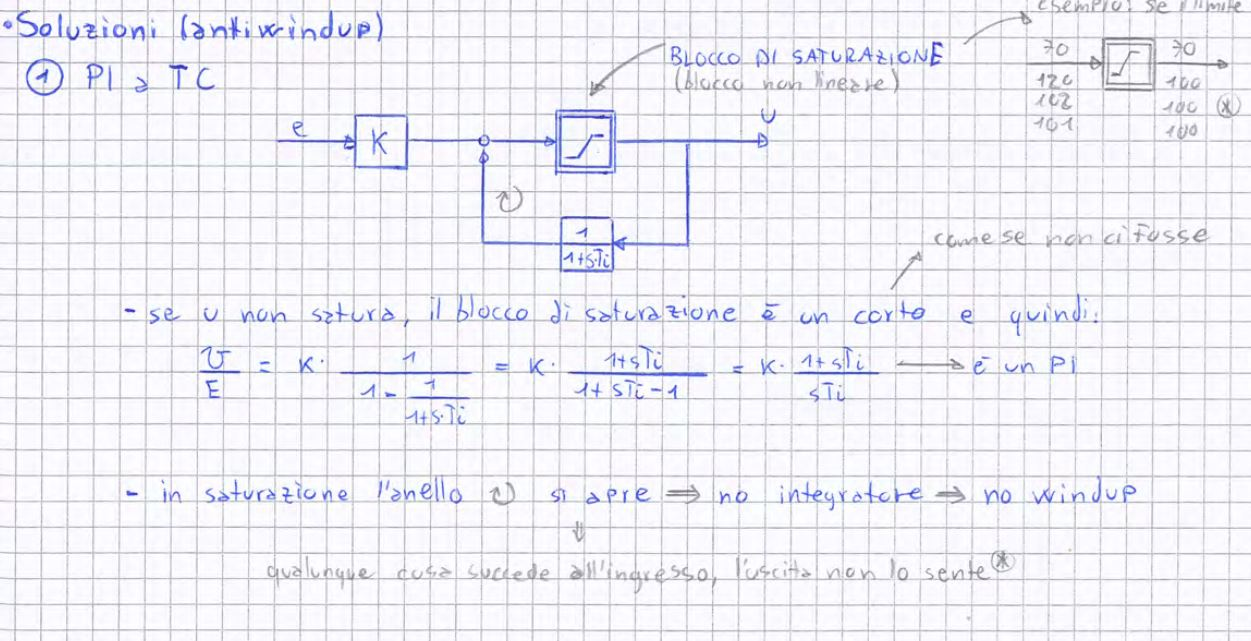
\includegraphics[height=4cm]{../formulario/img11.JPG}
        \end{center}
        \item Generico controllore a TD: \begin{center}
            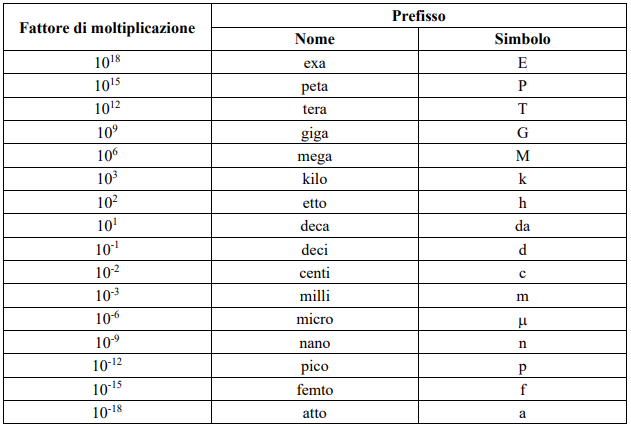
\includegraphics[height=5cm]{../formulario/img12.jpg}
        \end{center}
    \end{itemize}  
    \end{multicols*}
    \newpage
\begin{multicols*}{3}
\textbf{Lagrange TC}
\[
    x(t) = x_L(t) + x_F(t) =e^{At} x(0) + \int_{0}^{t}e^{A(t-\tau)}bu(\tau)d \tau
\]
\[
    y(t) 1 = y_L(t) + y_F(t) = ce^{At}x(0) + c \int_{0}^{t}e^{A(t-\tau)}bu(\tau)d \tau + du(t)
\]
\textbf{Lagrange TD}
\[
    x(k)= x_L(k) + x_F(k) =A^k x(0) + \sum_{l=0}^{k-1}A^{k-l-1}bu(l)
\]
\[
    y(k) = y_L(k) + y_F(k) = cx(k)+du(k) =cA^k x(0) + c\sum_{l=0}^{k-1}A^{k-l-1}bu(l) + du(k)
\]
\textbf{Esponenziale di matrice}
\[
    e^{At} = e^{TDT^{-1} t} = T e^{Dt} T^{-1} = \dots
\]
\textbf{Stabilità a TC:}
\begin{itemize}
    \item Tutti gli autovalori di $A$ hanno $Re < 0 \Longleftrightarrow $ sistema AS;
    \item Almeno un autovalore di $A$ ha $Re > 0 \Longrightarrow$ sistema I;
    \item Tutti gli autovalori di $A$ hanno $Re \leq 0$ e ne esiste almeno uno con $Re = 0$ $\Longrightarrow$ $\begin{cases}
        \text{sistema I; (mov lib diverge per t -> inf)}\;\\
        \text{oppure sistema S (mov lib limitato per t -> inf), ma non AS.}\;
    \end{cases}$.
\end{itemize}
\textbf{Stabilità a TD:}
\begin{itemize}
    \item Tutti gli autovalori di $A$ hanno $|\lambda_i| < 1$ $\Longleftrightarrow$ sistema AS.
    \item Almeno un autovalore di $A$ con modulo $|\lambda_i| > 1$ $\Longrightarrow$ sistema I.
    \item Tutti gli autovalori di $A$ hanno $|\lambda_i| \leq 1$ e ne esiste almeno uno tale che $|\lambda_1| = 1$ $\Longrightarrow$ $\begin{cases}
        \text{sistema I;}\;\\
        \text{oppure sistema S, ma non AS.}\;
    \end{cases}$.
\end{itemize}
\textbf{Stabilità e A:}
\begin{itemize}
    \item se $det(A) = 0$ esiste $S_i = 0$ $\Longrightarrow$ no AS.
    \item se $tr(A) >0$ $\Longrightarrow$ sistema I.
    \item se $tr(A) = 0$ $\Longrightarrow$ no AS.
    \item Se $Re(S_i)<0$ per ogni $i$ (cioè se il sistema è asintoticamente stabile), allora i coefficienti di $\Pi(S)$ sono tutti concordi e non nulli \newline
    \textbf{oss.} Errore tipico: il viceversa vale solo per polinomi del secondo ordine.
\end{itemize}
\textbf{Routh:}
\[
    w_i = - \frac{1}{q_1} det\left[\begin{matrix}
        h_1 & h_{i+1} \\
        q_1 & q_{i+1}
    \end{matrix}\right]
\]
\textbf{Trasformata di Laplace}\newline
Ritardo: $\mathcal{L}[ v(t - \tau)] = e^{-s \tau} \mathcal{L}[v(t)]$ (spesso utilizzata al contrario per Heaviside: $\mathcal{L}^{-1}\left[\frac{N(s)}{D(s)}e^{-s \tau}\right] \rightarrow $ Heaviside di $\frac{N(s)}{D(s)}$ ottengo $y(t)$, poi con $e^{-s \tau}$ aggiungo ritardo $\tau$ e $\rightarrow  y(t- \tau)$)
\renewcommand{\arraystretch}{2}
    \begin{center}
        \begin{tabular}{ |c|c| } 
        \hline
        \;\;\;\;\;\;\;\;\;\;\;\;\;\;\;$v(t)$ \;\;\;\;\;\;\;\;\;\;\;\;\;\;\;& \;\;\;\;\;\;\;\;\;\;\;\;\;\;\;$V(s)$ \;\;\;\;\;\;\;\;\;\;\;\;\;\;\;\\ 
        \hline
        $k \cdot imp(t)$ & $k \cdot 1$ \\ 
        $k \cdot sca(t)$ & $k \cdot \frac{1}{s}$  \\ 
        $k \cdot ram(t) =k \cdot t \cdot  sca(t)$ & $k \cdot \frac{1}{s^2}$ \\
        $k \cdot e^{at}sca(t)$ & $k \cdot \frac{1}{s-a}$ \\ 
        $t^{n}\cdot e^{at}sca(t)$ & $\frac{n!}{(s-a)^{n+1}}$\\ 
        $\frac{1}{(n-1)!} t^{n-1}e^{-at}$ & $\frac{1}{(s+a)^n}$\\
        \hline
        \end{tabular}
    \end{center}
    \renewcommand{\arraystretch}{1}
Teorema del valore finale: Se $V(s) = \mathcal{L}[v(t)]$ ed esiste $\lim_{t\rightarrow +\infty} v(t)$ o equivalentemente $V(s)$ ha solo poli con $Re< 0$ o nell'origine, allora $\lim_{t\rightarrow +\infty} v(t) = \lim_{s\rightarrow 0} s \cdot V(s)$.\newline
\textbf{Funzione di Trasferimento:}
\[
    X(s) = X_L(s) + X_F(s)
\]
\[
    \begin{cases}
        X_L(s) = (sI-A)^{-1} x(0)\\
        X_F(s) = (sI-A) ^{-1} b U(s)
    \end{cases}
\]
\[
    Y(s) = cX(s) + dU(s) = Y_L(s) + Y_F(s)
\]
\[
    \begin{cases}
        Y_L(s) = c(sI-A)^{-1} x(0)\\
        Y_F(s) = [c(sI-A)^{-1} b + d]U(s)
    \end{cases}
\]
Spesso può essere utile calcolare la $Y_F(s)$ a partire dall'equazione $\frac{Y(s)}{U(s)} = G(s)$
\[
    G(s) := c(sI-A)^{-1} b + d
\]
\textbf{Raggiungibilità:}
\[
    M_R= \;\text{matrice di raggiungibilità}\; =\left[\begin{matrix}
        b & Ab & A^2 b & \dots & A^{n-1}b
    \end{matrix}\right]
\] 
\textbf{Osservabilità:}
\[
    M_O = \left[\begin{matrix}
        c' & A'c' & \dots & (A^{n-1})' c'
    \end{matrix}\right]
\]
\textbf{Diagramma di Bode del modulo}: 
\begin{enumerate}
    \item Tracciare il diagramma di Bode del modulo di $\frac{\mu}{s^g}$ (è una retta la cui pendenza viene ricavata da: $-20 \cdot g \frac{dB}{decade}$; per capire dove interseca l'asse delle $\omega$ basta ricavare il valore di $\omega$ per cui $\left| \frac{\mu}{\omega^g} \right| = 1$; se la retta non ha pendenza allora è una retta orizzontale all'altezza di $|\mu|_{dB}$).
    \item Segnare sull'asse delle $\omega$ le frequenze d'angolo dei poli (radici del denominatore) e zeri (radici del numeratore) non in $s=0$ (perchè son già presenti nel punto precedente).\newline
    Quando si incontra una frequenza d'angolo di uno zero, la pendenza aumenta di $1$, quando si incontra una frequenza d'angolo di un polo, la pendenza diminuisce di $1$. (Ricordiamo che per 1 di pendenza si intendono $20 dB/decade$).
\end{enumerate}
\textbf{Diagramma di Bode della fase}:
\begin{enumerate}
    \item Il diagramma di Bode della fase parte al valore di $arg(\frac{\mu}{(j \omega)^g})$, che è calcolabile sommando i contributi di $\mu$ e $\frac{1}{s^g}$ nel seguente modo:
    \[
        \mu \rightarrow \begin{cases}
            0^o \;\;\;& se > 0\\
            -180^o \;\;\; & se <0
        \end{cases} \;\;\;\;\;\;\;\;\;\;\;\;\;\;\; \frac{1}{s^g}\rightarrow -g \cdot 90^o
    \]
    \item zero "a sinistra" la fase aumenta di $90^o$;\newline
    zero "a destra" la fase diminuisce di $90^o$;\newline
    polo "a sinistra" la fase diminuisce di $90^o$;\newline
    polo "a destra" la fase aumenta di $90^o$.
\end{enumerate}
\textbf{Trasformata Zeta:}
\begin{itemize}
    \item impulso: $\mathcal{Z}[imp(k)] = 1$
    \item scalino: $\mathcal{Z}[sca(k)] = \frac{z}{z-1}$ per $|z|>1$
    \item esponenziale: $\mathcal{Z}[a^k sca(k)] = \frac{z}{z-a}$ per $|z| > |a|$
\end{itemize}
\[
    X(z) = (zI-A)^{-1} z x(0) + (zI-A)^{-1} b U(z)
\]
\[
    Y(z) = cX(z) + dU(z) = c(zI-A)^{-1} z x(0) + [c(zI-A)^{-1} b + d] U(z)
\]
\[
    c(zI-A)^{-1} b + d
\]
\textbf{Scelta $T_s$:}
\[
    \omega_S =\frac{2\pi}{T_s} = \text{"\textbf{frequenza di campionamento}"}
\]
\[
    \omega_N = \frac{\omega_s}{2} = \text{\textbf{frequenza di Nyquist}}
\]
Quindi per trovare $\omega_s$ si traccia (nel diagramma di Bode del modulo di $L(s)$) la riga orizzontale a cui si vuole il $|L(j \omega_N)|$, dove interseca $|L|$ ci sarà la frequenza $\omega_N$, si moltiplica per due e si trova $\omega_s$.\newline
Il sempling and hold introduce un ritardo che influenza solo $\phi_m$: $\omega_c \frac{T_s}{2} < $ di un certo valore (da notare che $\omega_c \frac{T_s}{2}$ è in radianti !).\newline
Ritardi di calcolo:
\begin{itemize}
    \item caso 1: $\tau_c$ è variabile, ma molto minore di $T_s$ (tutto ok);
    \item caso 2: $\tau_c$ costante, ma non trascurabile rispetto a $T_s$ (problema);
    \item caso 3: $\tau_c$ variabile e non trascurabile rispetto a $T_s$ (problema);
\end{itemize}
Soluzione:
\begin{itemize}
    \item (caso 1) se solo effetto sampling and hold e ritardo calcolabile trascurabile, allora $\frac{1}{2} \omega_c T_s <$ un certo valore.
    \item (caso 2 e 3) se ritardo del calcolo non trascurabile, allora $\frac{3}{2} \omega_c T_S <$ un certo valore.
\end{itemize}
\textbf{Discretizzazione approssimata:}
\begin{itemize}
    \item Approssimazione 1: metodo di \textbf{Eulero esplicito} o delle differenze in avanti $R^*(z) = R\left(\frac{z-1}{T_s}\right)$;
    \item Approssimazione 2: metodo di \textbf{Eulero implicito} o delle differenze all'indietro $R^*(z) = R\left(\frac{1-z^{-1}}{T_s}\right) = R\left(\frac{z-1}{z T_s}\right)$
\end{itemize}
\textbf{Tustin:}
\[
    R^*(z) = R( \frac{2}{T_s} \cdot \frac{z-1}{z+1})
\]
\textbf{Da $R^*(z)$ alla legge di controllo a TD:}\newline
$R^*(z) = $ che d'ora in poi indichiamo solo come $R(z) = \frac{2z^2 - 3z +4}{z^2 -z}$. 
\begin{itemize}
    \item Perchè sia realizzabile l'unico vincolo è che il grado del numeratore sia minore o uguale al grado del denominatore.
    \item  Detto $U(z)$ l'uscita di $R(z)$ e $E(z)$ l'ingresso di $R(z)$, sappiamo che $\frac{U(z)}{E(z)} = R(z) = \frac{2z^2 - 3z +4}{z^2 -z}$.
    \item Tolgo i denominatori: $(z^2-z) U(z) = (2z^2 -3z+4) E(z)$.
    \item Ridistribuisco il prodotto: $z^2 U(z) - z U(z) = 2z^2 E(z) - 3zE(z) + 4 E(z)$.
    \item Antitrasformo (condizioni iniziali nulle): $u(k+2) - u(k+1) = 2e(k+2) -3e(k+1) + 4e(k)$.
    \item Risolvo per "l'uscita più recente" e scalo i tempi: in questo caso quella più recente è $u(k+2)$, quindi $u(k) = u(k-1) + 2 e(k) -3e(k-1) + 4e(k-2)$.
    \item Quindi, usando come convenzione "detta la generica variabile $x_n := x(k-n)$", possiamo scrivere il seguente algoritmo di controllo per ogni $T_s$:
    \begin{itemize}
        \item ottieni $e$;
        \item $u = u_1 +  2e - 3e_1 + 4e_2$;
        \item $e_2 = e_1$;
        \item $e_1 = e$;
        \item $u_1 = u$;
        \item applica $u$.
    \end{itemize}
\end{itemize}

\end{multicols*}
\end{landscape}